\documentclass[twoside]{book}

% Packages required by doxygen
\usepackage{fixltx2e}
\usepackage{calc}
\usepackage{doxygen}
\usepackage[export]{adjustbox} % also loads graphicx
\usepackage{graphicx}
\usepackage[utf8]{inputenc}
\usepackage{makeidx}
\usepackage{multicol}
\usepackage{multirow}
\PassOptionsToPackage{warn}{textcomp}
\usepackage{textcomp}
\usepackage[nointegrals]{wasysym}
\usepackage[table]{xcolor}

% Font selection
\usepackage[T1]{fontenc}
\usepackage[scaled=.90]{helvet}
\usepackage{courier}
\usepackage{amssymb}
\usepackage{sectsty}
\renewcommand{\familydefault}{\sfdefault}
\allsectionsfont{%
  \fontseries{bc}\selectfont%
  \color{darkgray}%
}
\renewcommand{\DoxyLabelFont}{%
  \fontseries{bc}\selectfont%
  \color{darkgray}%
}
\newcommand{\+}{\discretionary{\mbox{\scriptsize$\hookleftarrow$}}{}{}}

% Page & text layout
\usepackage{geometry}
\geometry{%
  a4paper,%
  top=2.5cm,%
  bottom=2.5cm,%
  left=2.5cm,%
  right=2.5cm%
}
\tolerance=750
\hfuzz=15pt
\hbadness=750
\setlength{\emergencystretch}{15pt}
\setlength{\parindent}{0cm}
\setlength{\parskip}{0.2cm}
\makeatletter
\renewcommand{\paragraph}{%
  \@startsection{paragraph}{4}{0ex}{-1.0ex}{1.0ex}{%
    \normalfont\normalsize\bfseries\SS@parafont%
  }%
}
\renewcommand{\subparagraph}{%
  \@startsection{subparagraph}{5}{0ex}{-1.0ex}{1.0ex}{%
    \normalfont\normalsize\bfseries\SS@subparafont%
  }%
}
\makeatother

% Headers & footers
\usepackage{fancyhdr}
\pagestyle{fancyplain}
\fancyhead[LE]{\fancyplain{}{\bfseries\thepage}}
\fancyhead[CE]{\fancyplain{}{}}
\fancyhead[RE]{\fancyplain{}{\bfseries\leftmark}}
\fancyhead[LO]{\fancyplain{}{\bfseries\rightmark}}
\fancyhead[CO]{\fancyplain{}{}}
\fancyhead[RO]{\fancyplain{}{\bfseries\thepage}}
\fancyfoot[LE]{\fancyplain{}{}}
\fancyfoot[CE]{\fancyplain{}{}}
\fancyfoot[RE]{\fancyplain{}{\bfseries\scriptsize Generated on Thu Dec 17 2015 14\+:25\+:09 for Y\+A\+H\+A\+L by Doxygen }}
\fancyfoot[LO]{\fancyplain{}{\bfseries\scriptsize Generated on Thu Dec 17 2015 14\+:25\+:09 for Y\+A\+H\+A\+L by Doxygen }}
\fancyfoot[CO]{\fancyplain{}{}}
\fancyfoot[RO]{\fancyplain{}{}}
\renewcommand{\footrulewidth}{0.4pt}
\renewcommand{\chaptermark}[1]{%
  \markboth{#1}{}%
}
\renewcommand{\sectionmark}[1]{%
  \markright{\thesection\ #1}%
}

% Indices & bibliography
\usepackage{natbib}
\usepackage[titles]{tocloft}
\setcounter{tocdepth}{3}
\setcounter{secnumdepth}{5}
\makeindex

% Hyperlinks (required, but should be loaded last)
\usepackage{ifpdf}
\ifpdf
  \usepackage[pdftex,pagebackref=true]{hyperref}
\else
  \usepackage[ps2pdf,pagebackref=true]{hyperref}
\fi
\hypersetup{%
  colorlinks=true,%
  linkcolor=blue,%
  citecolor=blue,%
  unicode%
}

% Custom commands
\newcommand{\clearemptydoublepage}{%
  \newpage{\pagestyle{empty}\cleardoublepage}%
}


%===== C O N T E N T S =====

\begin{document}

% Titlepage & ToC
\hypersetup{pageanchor=false,
             bookmarks=true,
             bookmarksnumbered=true,
             pdfencoding=unicode
            }
\pagenumbering{roman}
\begin{titlepage}
\vspace*{7cm}
\begin{center}%
{\Large Y\+A\+H\+A\+L }\\
\vspace*{1cm}
{\large Generated by Doxygen 1.8.10}\\
\vspace*{0.5cm}
{\small Thu Dec 17 2015 14:25:09}\\
\end{center}
\end{titlepage}
\clearemptydoublepage
\tableofcontents
\clearemptydoublepage
\pagenumbering{arabic}
\hypersetup{pageanchor=true}

%--- Begin generated contents ---
\chapter{yahal}
\label{md__home_andy__documentos__source_yahal__r_e_a_d_m_e}
\hypertarget{md__home_andy__documentos__source_yahal__r_e_a_d_m_e}{}
Yet Another Hardware Abstraction Layer (Y\+A\+H\+A\+L) 
\chapter{Namespace Index}
\section{Namespace List}
Here is a list of all namespaces with brief descriptions\+:\begin{DoxyCompactList}
\item\contentsline{section}{\hyperlink{namespaceerror}{error} }{\pageref{namespaceerror}}{}
\item\contentsline{section}{\hyperlink{namespacehal}{hal} \\*-\/--- I\+N\+C\+L\+U\+D\+E -\/-\/-\/-\/-\/-\/-\/-\/-\/-\/-\/-\/-\/-\/-\/-\/-\/-\/-\/-\/-\/-\/-\/-\/-\/-\/-\/-\/-\/-\/-\/-\/-\/-\/-\/-\/-\/-\/-\/-\/-\/-\/-\/-\/-\/-\/-\/-\/-\/-\/-\/-\/-\/-\/-\/-\/-\/-\/-\/-\/-\/-\/-\/-\/-\/-\/-\/-\/-\/-\/-\/-\/-\/------ }{\pageref{namespacehal}}{}
\item\contentsline{section}{\hyperlink{namespacehal_1_1utility}{hal\+::utility} }{\pageref{namespacehal_1_1utility}}{}
\item\contentsline{section}{\hyperlink{namespaceyahal}{yahal} }{\pageref{namespaceyahal}}{}
\item\contentsline{section}{\hyperlink{namespaceyahal_1_1mcu}{yahal\+::mcu} }{\pageref{namespaceyahal_1_1mcu}}{}
\end{DoxyCompactList}

\chapter{Hierarchical Index}
\section{Class Hierarchy}
This inheritance list is sorted roughly, but not completely, alphabetically\+:\begin{DoxyCompactList}
\item \contentsline{section}{hal\+:\+:sensors\+:\+:Ads1115}{\pageref{classhal_1_1sensors_1_1_ads1115}}{}
\item \contentsline{section}{hal\+:\+:battery\+:\+:Bq24193}{\pageref{classhal_1_1battery_1_1_bq24193}}{}
\item \contentsline{section}{yahal\+:\+:utility\+:\+:oop\+:\+:Callback$<$ T\+\_\+\+A\+R\+G\+U\+M\+E\+N\+T $>$}{\pageref{classyahal_1_1utility_1_1oop_1_1_callback}}{}
\item \contentsline{section}{yahal\+:\+:utility\+:\+:oop\+:\+:Callback$<$ Direction\+:\+:Type $>$}{\pageref{classyahal_1_1utility_1_1oop_1_1_callback}}{}
\item \contentsline{section}{yahal\+:\+:utility\+:\+:oop\+:\+:Callback$<$ uint8\+\_\+t \& $>$}{\pageref{classyahal_1_1utility_1_1oop_1_1_callback}}{}
\item \contentsline{section}{yahal\+:\+:utility\+:\+:oop\+:\+:Callback$<$ uint8\+\_\+t $>$}{\pageref{classyahal_1_1utility_1_1oop_1_1_callback}}{}
\item \contentsline{section}{yahal\+:\+:utility\+:\+:oop\+:\+:Callback$<$ void $>$}{\pageref{classyahal_1_1utility_1_1oop_1_1_callback_3_01void_01_4}}{}
\item \contentsline{section}{hal\+:\+:utility\+:\+:Counter$<$ T $>$}{\pageref{classhal_1_1utility_1_1_counter}}{}
\item \contentsline{section}{hal\+:\+:sensors\+:\+:Ads1115\+:\+:D\+A\+T\+A\+\_\+\+R\+A\+T\+E}{\pageref{structhal_1_1sensors_1_1_ads1115_1_1_d_a_t_a___r_a_t_e}}{}
\item \contentsline{section}{hal\+:\+:battery\+:\+:Bq24193\+:\+:D\+A\+T\+A\+\_\+\+R\+A\+T\+E}{\pageref{structhal_1_1battery_1_1_bq24193_1_1_d_a_t_a___r_a_t_e}}{}
\item \contentsline{section}{yahal\+:\+:mcu\+:\+:Gpio\+:\+:Direction}{\pageref{structyahal_1_1mcu_1_1_gpio_1_1_direction}}{}
\item \contentsline{section}{yahal\+:\+:mcu\+:\+:details\+:\+:I2\+C\+\_\+common\+:\+:Direction}{\pageref{structyahal_1_1mcu_1_1details_1_1_i2_c__common_1_1_direction}}{}
\item \contentsline{section}{yahal\+:\+:mcu\+:\+:Gpio\+:\+:Error}{\pageref{structyahal_1_1mcu_1_1_gpio_1_1_error}}{}
\item \contentsline{section}{yahal\+:\+:mcu\+:\+:Clk\+:\+:Error}{\pageref{structyahal_1_1mcu_1_1_clk_1_1_error}}{}
\item \contentsline{section}{yahal\+:\+:mcu\+:\+:Irq\+:\+:Error}{\pageref{structyahal_1_1mcu_1_1_irq_1_1_error}}{}
\item \contentsline{section}{yahal\+:\+:mcu\+:\+:Wdt\+:\+:Error}{\pageref{structyahal_1_1mcu_1_1_wdt_1_1_error}}{}
\item \contentsline{section}{yahal\+:\+:mcu\+:\+:details\+:\+:I2\+C\+\_\+common\+:\+:Error}{\pageref{structyahal_1_1mcu_1_1details_1_1_i2_c__common_1_1_error}}{}
\item \contentsline{section}{yahal\+:\+:error\+:\+:Error\+Code}{\pageref{classyahal_1_1error_1_1_error_code}}{}
\begin{DoxyCompactList}
\item \contentsline{section}{yahal\+:\+:mcu\+:\+:details\+:\+:Base\+Module}{\pageref{classyahal_1_1mcu_1_1details_1_1_base_module}}{}
\begin{DoxyCompactList}
\item \contentsline{section}{yahal\+:\+:mcu\+:\+:Clk}{\pageref{classyahal_1_1mcu_1_1_clk}}{}
\begin{DoxyCompactList}
\item \contentsline{section}{yahal\+:\+:mcu\+:\+:targets\+:\+:msp430f5309\+:\+:Clk}{\pageref{classyahal_1_1mcu_1_1targets_1_1msp430f5309_1_1_clk}}{}
\end{DoxyCompactList}
\item \contentsline{section}{yahal\+:\+:mcu\+:\+:details\+:\+:I2\+C\+\_\+common}{\pageref{classyahal_1_1mcu_1_1details_1_1_i2_c__common}}{}
\begin{DoxyCompactList}
\item \contentsline{section}{yahal\+:\+:mcu\+:\+:I2\+C\+\_\+master}{\pageref{classyahal_1_1mcu_1_1_i2_c__master}}{}
\item \contentsline{section}{yahal\+:\+:mcu\+:\+:I2\+C\+\_\+slave}{\pageref{classyahal_1_1mcu_1_1_i2_c__slave}}{}
\end{DoxyCompactList}
\item \contentsline{section}{yahal\+:\+:mcu\+:\+:Gpio}{\pageref{classyahal_1_1mcu_1_1_gpio}}{}
\begin{DoxyCompactList}
\item \contentsline{section}{yahal\+:\+:mcu\+:\+:targets\+:\+:msp430f5309\+:\+:Gpio}{\pageref{classyahal_1_1mcu_1_1targets_1_1msp430f5309_1_1_gpio}}{}
\end{DoxyCompactList}
\item \contentsline{section}{yahal\+:\+:mcu\+:\+:Irq}{\pageref{classyahal_1_1mcu_1_1_irq}}{}
\item \contentsline{section}{yahal\+:\+:mcu\+:\+:Wdt}{\pageref{classyahal_1_1mcu_1_1_wdt}}{}
\begin{DoxyCompactList}
\item \contentsline{section}{yahal\+:\+:mcu\+:\+:targets\+:\+:msp430f5309\+:\+:Wdt}{\pageref{classyahal_1_1mcu_1_1targets_1_1msp430f5309_1_1_wdt}}{}
\end{DoxyCompactList}
\end{DoxyCompactList}
\end{DoxyCompactList}
\item \contentsline{section}{yahal\+:\+:mcu\+:\+:targets\+:\+:msp430f5309\+:\+:Clk\+:\+:Frequency}{\pageref{structyahal_1_1mcu_1_1targets_1_1msp430f5309_1_1_clk_1_1_frequency}}{}
\item \contentsline{section}{yahal\+:\+:mcu\+:\+:Irq\+:\+:G\+P\+I\+O}{\pageref{structyahal_1_1mcu_1_1_irq_1_1_g_p_i_o}}{}
\item \contentsline{section}{yahal\+:\+:mcu\+:\+:Irq\+:\+:I2\+C}{\pageref{structyahal_1_1mcu_1_1_irq_1_1_i2_c}}{}
\item \contentsline{section}{hal\+:\+:sensors\+:\+:Ads1115\+:\+:I\+N\+P\+U\+T}{\pageref{structhal_1_1sensors_1_1_ads1115_1_1_i_n_p_u_t}}{}
\item \contentsline{section}{hal\+:\+:utility\+:\+:Message\+Buffer$<$ T\+\_\+data, T\+\_\+buffer\+Size $>$}{\pageref{classhal_1_1utility_1_1_message_buffer}}{}
\item \contentsline{section}{hal\+:\+:utility\+:\+:Message\+Stack$<$ T\+\_\+data, T\+\_\+stack\+Size $>$}{\pageref{classhal_1_1utility_1_1_message_stack}}{}
\item \contentsline{section}{yahal\+:\+:utility\+:\+:oop\+:\+:Noncopyable}{\pageref{classyahal_1_1utility_1_1oop_1_1_noncopyable}}{}
\begin{DoxyCompactList}
\item \contentsline{section}{yahal\+:\+:mcu\+:\+:details\+:\+:Base\+Module}{\pageref{classyahal_1_1mcu_1_1details_1_1_base_module}}{}
\item \contentsline{section}{yahal\+:\+:rtos\+:\+:api\+:\+:Mutex}{\pageref{classyahal_1_1rtos_1_1api_1_1_mutex}}{}
\begin{DoxyCompactList}
\item \contentsline{section}{yahal\+:\+:rtos\+:\+:Mutex}{\pageref{classyahal_1_1rtos_1_1_mutex}}{}
\end{DoxyCompactList}
\end{DoxyCompactList}
\item \contentsline{section}{yahal\+:\+:mcu\+:\+:Gpio\+:\+:Port\+:\+:Pin}{\pageref{classyahal_1_1mcu_1_1_gpio_1_1_port_1_1_pin}}{}
\item \contentsline{section}{yahal\+:\+:mcu\+:\+:Gpio\+:\+:Port}{\pageref{classyahal_1_1mcu_1_1_gpio_1_1_port}}{}
\item \contentsline{section}{yahal\+:\+:mcu\+:\+:Gpio\+:\+:Resistor}{\pageref{structyahal_1_1mcu_1_1_gpio_1_1_resistor}}{}
\item \contentsline{section}{hal\+:\+:sensors\+:\+:Ads1115\+:\+:S\+C\+A\+L\+E}{\pageref{structhal_1_1sensors_1_1_ads1115_1_1_s_c_a_l_e}}{}
\item \contentsline{section}{hal\+:\+:utility\+:\+:Sliding\+Window$<$ T\+\_\+data, T\+\_\+buffer\+Size $>$}{\pageref{classhal_1_1utility_1_1_sliding_window}}{}
\item \contentsline{section}{yahal\+:\+:mcu\+:\+:Irq\+:\+:U\+A\+R\+T}{\pageref{structyahal_1_1mcu_1_1_irq_1_1_u_a_r_t}}{}
\end{DoxyCompactList}

\chapter{Class Index}
\section{Class List}
Here are the classes, structs, unions and interfaces with brief descriptions\+:\begin{DoxyCompactList}
\item\contentsline{section}{\hyperlink{classhal_1_1sensors_1_1_ads1115}{hal\+::sensors\+::\+Ads1115} \\*M\+M\+M\+M\+M\+M\+M\+M\+M\+M\+M\+M\+M\+M\+M\+M\+M\+M\+M\+M\+M\+M\+M\+M\+M\+M\+M\+M\+M\+M\+M\+M\+M\+M\+M\+M\+M\+M\+M\+M\+M\+M\+M\+M\+M\+M\+M\+M\+M\+M\+M\+M\+M\+M\+M\+M\+M\+M\+M\+M\+M\+M\+M\+M\+M\+M\+M\+M\+M\+M\+M\+M\+M\+M\+M\+M\+M\+M\+M\+M\+M\+M\+M\+M\+M\+M\+M\+M\+M\+M\+M\+M\+M\+M\+M\+M\+M G\+P\+I\+O W\+W\+W\+W\+W\+W\+W\+W\+W\+W\+W\+W\+W\+W\+W\+W\+W\+W\+W\+W\+W\+W\+W\+W\+W\+W\+W\+W\+W\+W\+W\+W\+W\+W\+W\+W\+W\+W\+W\+W\+W\+W\+W\+W\+W\+W\+W\+W\+W\+W\+W\+W\+W\+W\+W\+W\+W\+W\+W\+W\+W\+W\+W\+W\+W\+W\+W\+W\+W\+W\+W\+W\+W\+W\+W\+W\+W\+W\+W\+W\+W\+W\+W\+W\+W\+W\+W\+W\+W\+W\+W\+W\+W\+W\+W\+W }{\pageref{classhal_1_1sensors_1_1_ads1115}}{}
\item\contentsline{section}{\hyperlink{classyahal_1_1mcu_1_1details_1_1_base_module}{yahal\+::mcu\+::details\+::\+Base\+Module} \\*Base class for all M\+C\+U modules }{\pageref{classyahal_1_1mcu_1_1details_1_1_base_module}}{}
\item\contentsline{section}{\hyperlink{classhal_1_1battery_1_1_bq24193}{hal\+::battery\+::\+Bq24193} \\*M\+M\+M\+M\+M\+M\+M\+M\+M\+M\+M\+M\+M\+M\+M\+M\+M\+M\+M\+M\+M\+M\+M\+M\+M\+M\+M\+M\+M\+M\+M\+M\+M\+M\+M\+M\+M\+M\+M\+M\+M\+M\+M\+M\+M\+M\+M\+M\+M\+M\+M\+M\+M\+M\+M\+M\+M\+M\+M\+M\+M\+M\+M\+M\+M\+M\+M\+M\+M\+M\+M\+M\+M\+M\+M\+M\+M\+M\+M\+M\+M\+M\+M\+M\+M\+M\+M\+M\+M\+M\+M\+M\+M\+M\+M\+M\+M G\+P\+I\+O W\+W\+W\+W\+W\+W\+W\+W\+W\+W\+W\+W\+W\+W\+W\+W\+W\+W\+W\+W\+W\+W\+W\+W\+W\+W\+W\+W\+W\+W\+W\+W\+W\+W\+W\+W\+W\+W\+W\+W\+W\+W\+W\+W\+W\+W\+W\+W\+W\+W\+W\+W\+W\+W\+W\+W\+W\+W\+W\+W\+W\+W\+W\+W\+W\+W\+W\+W\+W\+W\+W\+W\+W\+W\+W\+W\+W\+W\+W\+W\+W\+W\+W\+W\+W\+W\+W\+W\+W\+W\+W\+W\+W\+W\+W\+W }{\pageref{classhal_1_1battery_1_1_bq24193}}{}
\item\contentsline{section}{\hyperlink{classyahal_1_1utility_1_1oop_1_1_callback}{yahal\+::utility\+::oop\+::\+Callback$<$ T\+\_\+\+A\+R\+G\+U\+M\+E\+N\+T $>$} \\*============================================================================== W\+I\+T\+H A\+R\+G\+U\+M\+E\+N\+T }{\pageref{classyahal_1_1utility_1_1oop_1_1_callback}}{}
\item\contentsline{section}{\hyperlink{classyahal_1_1utility_1_1oop_1_1_callback_3_01void_01_4}{yahal\+::utility\+::oop\+::\+Callback$<$ void $>$} \\*=========================================================================== W\+I\+T\+H\+O\+U\+T A\+R\+G\+U\+M\+E\+N\+T }{\pageref{classyahal_1_1utility_1_1oop_1_1_callback_3_01void_01_4}}{}
\item\contentsline{section}{\hyperlink{classyahal_1_1mcu_1_1targets_1_1msp430f5309_1_1_clk}{yahal\+::mcu\+::targets\+::msp430f5309\+::\+Clk} \\*\begin{DoxyVerb}\end{DoxyVerb}
 }{\pageref{classyahal_1_1mcu_1_1targets_1_1msp430f5309_1_1_clk}}{}
\item\contentsline{section}{\hyperlink{classyahal_1_1mcu_1_1_clk}{yahal\+::mcu\+::\+Clk} \\*Base class for all system clock handling modules }{\pageref{classyahal_1_1mcu_1_1_clk}}{}
\item\contentsline{section}{\hyperlink{classhal_1_1utility_1_1_counter}{hal\+::utility\+::\+Counter$<$ T $>$} }{\pageref{classhal_1_1utility_1_1_counter}}{}
\item\contentsline{section}{\hyperlink{structhal_1_1sensors_1_1_ads1115_1_1_d_a_t_a___r_a_t_e}{hal\+::sensors\+::\+Ads1115\+::\+D\+A\+T\+A\+\_\+\+R\+A\+T\+E} }{\pageref{structhal_1_1sensors_1_1_ads1115_1_1_d_a_t_a___r_a_t_e}}{}
\item\contentsline{section}{\hyperlink{structhal_1_1battery_1_1_bq24193_1_1_d_a_t_a___r_a_t_e}{hal\+::battery\+::\+Bq24193\+::\+D\+A\+T\+A\+\_\+\+R\+A\+T\+E} }{\pageref{structhal_1_1battery_1_1_bq24193_1_1_d_a_t_a___r_a_t_e}}{}
\item\contentsline{section}{\hyperlink{structyahal_1_1mcu_1_1_gpio_1_1_direction}{yahal\+::mcu\+::\+Gpio\+::\+Direction} \\*\hyperlink{structyahal_1_1mcu_1_1_gpio_1_1_direction}{Direction} of G\+P\+I\+O pins }{\pageref{structyahal_1_1mcu_1_1_gpio_1_1_direction}}{}
\item\contentsline{section}{\hyperlink{structyahal_1_1mcu_1_1details_1_1_i2_c__common_1_1_direction}{yahal\+::mcu\+::details\+::\+I2\+C\+\_\+common\+::\+Direction} \\*I/\+O operation direction }{\pageref{structyahal_1_1mcu_1_1details_1_1_i2_c__common_1_1_direction}}{}
\item\contentsline{section}{\hyperlink{structyahal_1_1mcu_1_1_gpio_1_1_error}{yahal\+::mcu\+::\+Gpio\+::\+Error} \\*G\+P\+I\+O errors }{\pageref{structyahal_1_1mcu_1_1_gpio_1_1_error}}{}
\item\contentsline{section}{\hyperlink{structyahal_1_1mcu_1_1_clk_1_1_error}{yahal\+::mcu\+::\+Clk\+::\+Error} }{\pageref{structyahal_1_1mcu_1_1_clk_1_1_error}}{}
\item\contentsline{section}{\hyperlink{structyahal_1_1mcu_1_1_irq_1_1_error}{yahal\+::mcu\+::\+Irq\+::\+Error} }{\pageref{structyahal_1_1mcu_1_1_irq_1_1_error}}{}
\item\contentsline{section}{\hyperlink{structyahal_1_1mcu_1_1_wdt_1_1_error}{yahal\+::mcu\+::\+Wdt\+::\+Error} }{\pageref{structyahal_1_1mcu_1_1_wdt_1_1_error}}{}
\item\contentsline{section}{\hyperlink{structyahal_1_1mcu_1_1details_1_1_i2_c__common_1_1_error}{yahal\+::mcu\+::details\+::\+I2\+C\+\_\+common\+::\+Error} \\*\hyperlink{structyahal_1_1mcu_1_1details_1_1_i2_c__common_1_1_error}{Error} codes for I2\+C }{\pageref{structyahal_1_1mcu_1_1details_1_1_i2_c__common_1_1_error}}{}
\item\contentsline{section}{\hyperlink{classyahal_1_1error_1_1_error_code}{yahal\+::error\+::\+Error\+Code} \\*Base class for error code handling }{\pageref{classyahal_1_1error_1_1_error_code}}{}
\item\contentsline{section}{\hyperlink{structyahal_1_1mcu_1_1targets_1_1msp430f5309_1_1_clk_1_1_frequency}{yahal\+::mcu\+::targets\+::msp430f5309\+::\+Clk\+::\+Frequency} }{\pageref{structyahal_1_1mcu_1_1targets_1_1msp430f5309_1_1_clk_1_1_frequency}}{}
\item\contentsline{section}{\hyperlink{classyahal_1_1mcu_1_1targets_1_1msp430f5309_1_1_gpio}{yahal\+::mcu\+::targets\+::msp430f5309\+::\+Gpio} \\*\begin{DoxyVerb}\end{DoxyVerb}
 }{\pageref{classyahal_1_1mcu_1_1targets_1_1msp430f5309_1_1_gpio}}{}
\item\contentsline{section}{\hyperlink{structyahal_1_1mcu_1_1_irq_1_1_g_p_i_o}{yahal\+::mcu\+::\+Irq\+::\+G\+P\+I\+O} }{\pageref{structyahal_1_1mcu_1_1_irq_1_1_g_p_i_o}}{}
\item\contentsline{section}{\hyperlink{classyahal_1_1mcu_1_1_gpio}{yahal\+::mcu\+::\+Gpio} \\*Base class for G\+P\+I\+O modules }{\pageref{classyahal_1_1mcu_1_1_gpio}}{}
\item\contentsline{section}{\hyperlink{structyahal_1_1mcu_1_1_irq_1_1_i2_c}{yahal\+::mcu\+::\+Irq\+::\+I2\+C} }{\pageref{structyahal_1_1mcu_1_1_irq_1_1_i2_c}}{}
\item\contentsline{section}{\hyperlink{classyahal_1_1mcu_1_1details_1_1_i2_c__common}{yahal\+::mcu\+::details\+::\+I2\+C\+\_\+common} \\*Base class for all I2\+C modules }{\pageref{classyahal_1_1mcu_1_1details_1_1_i2_c__common}}{}
\item\contentsline{section}{\hyperlink{classyahal_1_1mcu_1_1_i2_c__master}{yahal\+::mcu\+::\+I2\+C\+\_\+master} \\*Base class for all I2\+C Masters }{\pageref{classyahal_1_1mcu_1_1_i2_c__master}}{}
\item\contentsline{section}{\hyperlink{classyahal_1_1mcu_1_1_i2_c__slave}{yahal\+::mcu\+::\+I2\+C\+\_\+slave} \\*Base class for all I2\+C slaves }{\pageref{classyahal_1_1mcu_1_1_i2_c__slave}}{}
\item\contentsline{section}{\hyperlink{structhal_1_1sensors_1_1_ads1115_1_1_i_n_p_u_t}{hal\+::sensors\+::\+Ads1115\+::\+I\+N\+P\+U\+T} }{\pageref{structhal_1_1sensors_1_1_ads1115_1_1_i_n_p_u_t}}{}
\item\contentsline{section}{\hyperlink{classyahal_1_1mcu_1_1_irq}{yahal\+::mcu\+::\+Irq} \\*Base class for all I\+R\+Q handlers }{\pageref{classyahal_1_1mcu_1_1_irq}}{}
\item\contentsline{section}{\hyperlink{classhal_1_1utility_1_1_message_buffer}{hal\+::utility\+::\+Message\+Buffer$<$ T\+\_\+data, T\+\_\+buffer\+Size $>$} }{\pageref{classhal_1_1utility_1_1_message_buffer}}{}
\item\contentsline{section}{\hyperlink{classhal_1_1utility_1_1_message_stack}{hal\+::utility\+::\+Message\+Stack$<$ T\+\_\+data, T\+\_\+stack\+Size $>$} }{\pageref{classhal_1_1utility_1_1_message_stack}}{}
\item\contentsline{section}{\hyperlink{classyahal_1_1rtos_1_1api_1_1_mutex}{yahal\+::rtos\+::api\+::\+Mutex} \\*Base class for all M\+U\+T\+E\+X }{\pageref{classyahal_1_1rtos_1_1api_1_1_mutex}}{}
\item\contentsline{section}{\hyperlink{classyahal_1_1rtos_1_1_mutex}{yahal\+::rtos\+::\+Mutex} \\*Does absolutely nothing }{\pageref{classyahal_1_1rtos_1_1_mutex}}{}
\item\contentsline{section}{\hyperlink{classyahal_1_1utility_1_1oop_1_1_noncopyable}{yahal\+::utility\+::oop\+::\+Noncopyable} \\*Non copyable base class }{\pageref{classyahal_1_1utility_1_1oop_1_1_noncopyable}}{}
\item\contentsline{section}{\hyperlink{classyahal_1_1mcu_1_1_gpio_1_1_port_1_1_pin}{yahal\+::mcu\+::\+Gpio\+::\+Port\+::\+Pin} \\*Base class for all G\+P\+I\+O Pins }{\pageref{classyahal_1_1mcu_1_1_gpio_1_1_port_1_1_pin}}{}
\item\contentsline{section}{\hyperlink{classyahal_1_1mcu_1_1_gpio_1_1_port}{yahal\+::mcu\+::\+Gpio\+::\+Port} \\*Base class for all G\+P\+I\+O Ports }{\pageref{classyahal_1_1mcu_1_1_gpio_1_1_port}}{}
\item\contentsline{section}{\hyperlink{structyahal_1_1mcu_1_1_gpio_1_1_resistor}{yahal\+::mcu\+::\+Gpio\+::\+Resistor} \\*Pull-\/up and pull-\/down resistor configuration }{\pageref{structyahal_1_1mcu_1_1_gpio_1_1_resistor}}{}
\item\contentsline{section}{\hyperlink{structhal_1_1sensors_1_1_ads1115_1_1_s_c_a_l_e}{hal\+::sensors\+::\+Ads1115\+::\+S\+C\+A\+L\+E} }{\pageref{structhal_1_1sensors_1_1_ads1115_1_1_s_c_a_l_e}}{}
\item\contentsline{section}{\hyperlink{classhal_1_1utility_1_1_sliding_window}{hal\+::utility\+::\+Sliding\+Window$<$ T\+\_\+data, T\+\_\+buffer\+Size $>$} }{\pageref{classhal_1_1utility_1_1_sliding_window}}{}
\item\contentsline{section}{\hyperlink{structyahal_1_1mcu_1_1_irq_1_1_u_a_r_t}{yahal\+::mcu\+::\+Irq\+::\+U\+A\+R\+T} }{\pageref{structyahal_1_1mcu_1_1_irq_1_1_u_a_r_t}}{}
\item\contentsline{section}{\hyperlink{classyahal_1_1mcu_1_1targets_1_1msp430f5309_1_1_wdt}{yahal\+::mcu\+::targets\+::msp430f5309\+::\+Wdt} \\*\begin{DoxyVerb}\end{DoxyVerb}
 }{\pageref{classyahal_1_1mcu_1_1targets_1_1msp430f5309_1_1_wdt}}{}
\item\contentsline{section}{\hyperlink{classyahal_1_1mcu_1_1_wdt}{yahal\+::mcu\+::\+Wdt} \\*Base class for all Watch Dog Timers }{\pageref{classyahal_1_1mcu_1_1_wdt}}{}
\end{DoxyCompactList}

\chapter{File Index}
\section{File List}
Here is a list of all documented files with brief descriptions\+:\begin{DoxyCompactList}
\item\contentsline{section}{/home/andy/\+Documentos/\+Source/yahal/error/{\bfseries error\+\_\+code.\+hpp} }{\pageref{error__code_8hpp}}{}
\item\contentsline{section}{/home/andy/\+Documentos/\+Source/yahal/error/\hyperlink{longjmp__exception_8hpp}{longjmp\+\_\+exception.\+hpp} \\*}{\pageref{longjmp__exception_8hpp}}{}
\item\contentsline{section}{/home/andy/\+Documentos/\+Source/yahal/error/{\bfseries trap.\+hpp} }{\pageref{trap_8hpp}}{}
\item\contentsline{section}{/home/andy/\+Documentos/\+Source/yahal/mcu/\hyperlink{mcu_8hpp}{mcu.\+hpp} \\*Main M\+C\+U file }{\pageref{mcu_8hpp}}{}
\item\contentsline{section}{/home/andy/\+Documentos/\+Source/yahal/mcu/config/{\bfseries mcu\+\_\+config.\+hpp} }{\pageref{mcu__config_8hpp}}{}
\item\contentsline{section}{/home/andy/\+Documentos/\+Source/yahal/mcu/config/hwemulation/{\bfseries hwemulation\+\_\+config.\+hpp} }{\pageref{config_2hwemulation_2hwemulation__config_8hpp}}{}
\item\contentsline{section}{/home/andy/\+Documentos/\+Source/yahal/mcu/config/targets/{\bfseries msp430f5309\+\_\+config.\+hpp} }{\pageref{msp430f5309__config_8hpp}}{}
\item\contentsline{section}{/home/andy/\+Documentos/\+Source/yahal/mcu/hwemulation/{\bfseries hwemulation.\+hpp} }{\pageref{hwemulation_8hpp}}{}
\item\contentsline{section}{/home/andy/\+Documentos/\+Source/yahal/mcu/hwemulation/{\bfseries hwemulation\+\_\+config.\+hpp} }{\pageref{hwemulation_2hwemulation__config_8hpp}}{}
\item\contentsline{section}{/home/andy/\+Documentos/\+Source/yahal/mcu/hwemulation/i2c/{\bfseries i2c\+\_\+master.\+cpp} }{\pageref{hwemulation_2i2c_2i2c__master_8cpp}}{}
\item\contentsline{section}{/home/andy/\+Documentos/\+Source/yahal/mcu/hwemulation/i2c/{\bfseries i2c\+\_\+master.\+hpp} }{\pageref{hwemulation_2i2c_2i2c__master_8hpp}}{}
\item\contentsline{section}{/home/andy/\+Documentos/\+Source/yahal/mcu/modules/\hyperlink{base__module_8hpp}{base\+\_\+module.\+hpp} }{\pageref{base__module_8hpp}}{}
\item\contentsline{section}{/home/andy/\+Documentos/\+Source/yahal/mcu/modules/\hyperlink{modules_8hpp}{modules.\+hpp} \\*Includes all modules }{\pageref{modules_8hpp}}{}
\item\contentsline{section}{/home/andy/\+Documentos/\+Source/yahal/mcu/modules/clk/{\bfseries clk.\+hpp} }{\pageref{modules_2clk_2clk_8hpp}}{}
\item\contentsline{section}{/home/andy/\+Documentos/\+Source/yahal/mcu/modules/gpio/{\bfseries gpio.\+cpp} }{\pageref{modules_2gpio_2gpio_8cpp}}{}
\item\contentsline{section}{/home/andy/\+Documentos/\+Source/yahal/mcu/modules/gpio/{\bfseries gpio.\+hpp} }{\pageref{modules_2gpio_2gpio_8hpp}}{}
\item\contentsline{section}{/home/andy/\+Documentos/\+Source/yahal/mcu/modules/i2c/{\bfseries i2c\+\_\+common.\+hpp} }{\pageref{i2c__common_8hpp}}{}
\item\contentsline{section}{/home/andy/\+Documentos/\+Source/yahal/mcu/modules/i2c/{\bfseries i2c\+\_\+master.\+cpp} }{\pageref{modules_2i2c_2i2c__master_8cpp}}{}
\item\contentsline{section}{/home/andy/\+Documentos/\+Source/yahal/mcu/modules/i2c/{\bfseries i2c\+\_\+master.\+hpp} }{\pageref{modules_2i2c_2i2c__master_8hpp}}{}
\item\contentsline{section}{/home/andy/\+Documentos/\+Source/yahal/mcu/modules/i2c/{\bfseries i2c\+\_\+multimaster.\+cpp} }{\pageref{modules_2i2c_2i2c__multimaster_8cpp}}{}
\item\contentsline{section}{/home/andy/\+Documentos/\+Source/yahal/mcu/modules/i2c/{\bfseries i2c\+\_\+multimaster.\+hpp} }{\pageref{modules_2i2c_2i2c__multimaster_8hpp}}{}
\item\contentsline{section}{/home/andy/\+Documentos/\+Source/yahal/mcu/modules/i2c/{\bfseries i2c\+\_\+slave.\+cpp} }{\pageref{modules_2i2c_2i2c__slave_8cpp}}{}
\item\contentsline{section}{/home/andy/\+Documentos/\+Source/yahal/mcu/modules/i2c/{\bfseries i2c\+\_\+slave.\+hpp} }{\pageref{modules_2i2c_2i2c__slave_8hpp}}{}
\item\contentsline{section}{/home/andy/\+Documentos/\+Source/yahal/mcu/modules/irq/{\bfseries irq.\+hpp} }{\pageref{modules_2irq_2irq_8hpp}}{}
\item\contentsline{section}{/home/andy/\+Documentos/\+Source/yahal/mcu/modules/uart/{\bfseries uart.\+cpp} }{\pageref{uart_8cpp}}{}
\item\contentsline{section}{/home/andy/\+Documentos/\+Source/yahal/mcu/modules/uart/{\bfseries uart.\+hpp} }{\pageref{uart_8hpp}}{}
\item\contentsline{section}{/home/andy/\+Documentos/\+Source/yahal/mcu/modules/wdt/{\bfseries wdt.\+hpp} }{\pageref{modules_2wdt_2wdt_8hpp}}{}
\item\contentsline{section}{/home/andy/\+Documentos/\+Source/yahal/mcu/targets/{\bfseries targets.\+hpp} }{\pageref{targets_8hpp}}{}
\item\contentsline{section}{/home/andy/\+Documentos/\+Source/yahal/mcu/targets/{\bfseries targets\+\_\+uid.\+hpp} }{\pageref{targets__uid_8hpp}}{}
\item\contentsline{section}{/home/andy/\+Documentos/\+Source/yahal/mcu/targets/msp430f2132/{\bfseries msp430f2132.\+hpp} }{\pageref{msp430f2132_8hpp}}{}
\item\contentsline{section}{/home/andy/\+Documentos/\+Source/yahal/mcu/targets/msp430f2132/{\bfseries msp430f2132\+\_\+config.\+hpp} }{\pageref{msp430f2132__config_8hpp}}{}
\item\contentsline{section}{/home/andy/\+Documentos/\+Source/yahal/mcu/targets/msp430f2132/{\bfseries msp430f2132\+\_\+modules.\+hpp} }{\pageref{msp430f2132__modules_8hpp}}{}
\item\contentsline{section}{/home/andy/\+Documentos/\+Source/yahal/mcu/targets/msp430f2132/clk/{\bfseries clk.\+cpp} }{\pageref{msp430f2132_2clk_2clk_8cpp}}{}
\item\contentsline{section}{/home/andy/\+Documentos/\+Source/yahal/mcu/targets/msp430f2132/clk/{\bfseries clk.\+hpp} }{\pageref{targets_2msp430f2132_2clk_2clk_8hpp}}{}
\item\contentsline{section}{/home/andy/\+Documentos/\+Source/yahal/mcu/targets/msp430f2132/gpio/{\bfseries gpio.\+cpp} }{\pageref{targets_2msp430f2132_2gpio_2gpio_8cpp}}{}
\item\contentsline{section}{/home/andy/\+Documentos/\+Source/yahal/mcu/targets/msp430f2132/gpio/{\bfseries gpio.\+hpp} }{\pageref{targets_2msp430f2132_2gpio_2gpio_8hpp}}{}
\item\contentsline{section}{/home/andy/\+Documentos/\+Source/yahal/mcu/targets/msp430f2132/i2c/{\bfseries i2c\+\_\+master.\+cpp} }{\pageref{targets_2msp430f2132_2i2c_2i2c__master_8cpp}}{}
\item\contentsline{section}{/home/andy/\+Documentos/\+Source/yahal/mcu/targets/msp430f2132/i2c/{\bfseries i2c\+\_\+master.\+hpp} }{\pageref{targets_2msp430f2132_2i2c_2i2c__master_8hpp}}{}
\item\contentsline{section}{/home/andy/\+Documentos/\+Source/yahal/mcu/targets/msp430f2132/i2c/{\bfseries i2c\+\_\+slave.\+cpp} }{\pageref{targets_2msp430f2132_2i2c_2i2c__slave_8cpp}}{}
\item\contentsline{section}{/home/andy/\+Documentos/\+Source/yahal/mcu/targets/msp430f2132/i2c/{\bfseries i2c\+\_\+slave.\+hpp} }{\pageref{targets_2msp430f2132_2i2c_2i2c__slave_8hpp}}{}
\item\contentsline{section}{/home/andy/\+Documentos/\+Source/yahal/mcu/targets/msp430f2132/irq/{\bfseries irq.\+cpp} }{\pageref{msp430f2132_2irq_2irq_8cpp}}{}
\item\contentsline{section}{/home/andy/\+Documentos/\+Source/yahal/mcu/targets/msp430f2132/irq/{\bfseries irq.\+hpp} }{\pageref{targets_2msp430f2132_2irq_2irq_8hpp}}{}
\item\contentsline{section}{/home/andy/\+Documentos/\+Source/yahal/mcu/targets/msp430f2132/wdt/{\bfseries wdt.\+cpp} }{\pageref{msp430f2132_2wdt_2wdt_8cpp}}{}
\item\contentsline{section}{/home/andy/\+Documentos/\+Source/yahal/mcu/targets/msp430f2132/wdt/{\bfseries wdt.\+hpp} }{\pageref{targets_2msp430f2132_2wdt_2wdt_8hpp}}{}
\item\contentsline{section}{/home/andy/\+Documentos/\+Source/yahal/mcu/targets/msp430f5309/{\bfseries msp430f5309.\+hpp} }{\pageref{msp430f5309_8hpp}}{}
\item\contentsline{section}{/home/andy/\+Documentos/\+Source/yahal/mcu/targets/msp430f5309/clk/{\bfseries clk.\+cpp} }{\pageref{msp430f5309_2clk_2clk_8cpp}}{}
\item\contentsline{section}{/home/andy/\+Documentos/\+Source/yahal/mcu/targets/msp430f5309/clk/{\bfseries clk.\+hpp} }{\pageref{targets_2msp430f5309_2clk_2clk_8hpp}}{}
\item\contentsline{section}{/home/andy/\+Documentos/\+Source/yahal/mcu/targets/msp430f5309/gpio/{\bfseries gpio.\+cpp} }{\pageref{targets_2msp430f5309_2gpio_2gpio_8cpp}}{}
\item\contentsline{section}{/home/andy/\+Documentos/\+Source/yahal/mcu/targets/msp430f5309/gpio/{\bfseries gpio.\+hpp} }{\pageref{targets_2msp430f5309_2gpio_2gpio_8hpp}}{}
\item\contentsline{section}{/home/andy/\+Documentos/\+Source/yahal/mcu/targets/msp430f5309/i2c/{\bfseries i2c\+\_\+master.\+cpp} }{\pageref{targets_2msp430f5309_2i2c_2i2c__master_8cpp}}{}
\item\contentsline{section}{/home/andy/\+Documentos/\+Source/yahal/mcu/targets/msp430f5309/i2c/{\bfseries i2c\+\_\+master.\+hpp} }{\pageref{targets_2msp430f5309_2i2c_2i2c__master_8hpp}}{}
\item\contentsline{section}{/home/andy/\+Documentos/\+Source/yahal/mcu/targets/msp430f5309/i2c/{\bfseries i2c\+\_\+multimaster.\+cpp} }{\pageref{targets_2msp430f5309_2i2c_2i2c__multimaster_8cpp}}{}
\item\contentsline{section}{/home/andy/\+Documentos/\+Source/yahal/mcu/targets/msp430f5309/i2c/{\bfseries i2c\+\_\+multimaster.\+hpp} }{\pageref{targets_2msp430f5309_2i2c_2i2c__multimaster_8hpp}}{}
\item\contentsline{section}{/home/andy/\+Documentos/\+Source/yahal/mcu/targets/msp430f5309/i2c/{\bfseries i2c\+\_\+slave.\+cpp} }{\pageref{targets_2msp430f5309_2i2c_2i2c__slave_8cpp}}{}
\item\contentsline{section}{/home/andy/\+Documentos/\+Source/yahal/mcu/targets/msp430f5309/i2c/{\bfseries i2c\+\_\+slave.\+hpp} }{\pageref{targets_2msp430f5309_2i2c_2i2c__slave_8hpp}}{}
\item\contentsline{section}{/home/andy/\+Documentos/\+Source/yahal/mcu/targets/msp430f5309/irq/{\bfseries irq.\+cpp} }{\pageref{msp430f5309_2irq_2irq_8cpp}}{}
\item\contentsline{section}{/home/andy/\+Documentos/\+Source/yahal/mcu/targets/msp430f5309/irq/{\bfseries irq.\+hpp} }{\pageref{targets_2msp430f5309_2irq_2irq_8hpp}}{}
\item\contentsline{section}{/home/andy/\+Documentos/\+Source/yahal/mcu/targets/msp430f5309/timer/{\bfseries timer.\+cpp} }{\pageref{timer_8cpp}}{}
\item\contentsline{section}{/home/andy/\+Documentos/\+Source/yahal/mcu/targets/msp430f5309/timer/{\bfseries timer.\+hpp} }{\pageref{timer_8hpp}}{}
\item\contentsline{section}{/home/andy/\+Documentos/\+Source/yahal/mcu/targets/msp430f5309/wdt/{\bfseries wdt.\+cpp} }{\pageref{msp430f5309_2wdt_2wdt_8cpp}}{}
\item\contentsline{section}{/home/andy/\+Documentos/\+Source/yahal/mcu/targets/msp430f5309/wdt/{\bfseries wdt.\+hpp} }{\pageref{targets_2msp430f5309_2wdt_2wdt_8hpp}}{}
\item\contentsline{section}{/home/andy/\+Documentos/\+Source/yahal/rtos/{\bfseries rtos.\+hpp} }{\pageref{rtos_8hpp}}{}
\item\contentsline{section}{/home/andy/\+Documentos/\+Source/yahal/rtos/{\bfseries rtos\+\_\+uid.\+hpp} }{\pageref{rtos__uid_8hpp}}{}
\item\contentsline{section}{/home/andy/\+Documentos/\+Source/yahal/rtos/api/{\bfseries api.\+hpp} }{\pageref{api_8hpp}}{}
\item\contentsline{section}{/home/andy/\+Documentos/\+Source/yahal/rtos/api/{\bfseries api\+\_\+mutex.\+hpp} }{\pageref{api__mutex_8hpp}}{}
\item\contentsline{section}{/home/andy/\+Documentos/\+Source/yahal/rtos/implementations/single\+\_\+thread/{\bfseries st.\+hpp} }{\pageref{st_8hpp}}{}
\item\contentsline{section}{/home/andy/\+Documentos/\+Source/yahal/rtos/implementations/single\+\_\+thread/{\bfseries st\+\_\+mutex.\+hpp} }{\pageref{st__mutex_8hpp}}{}
\item\contentsline{section}{/home/andy/\+Documentos/\+Source/yahal/sensors/ads1115/{\bfseries ads1115.\+cpp} }{\pageref{ads1115_8cpp}}{}
\item\contentsline{section}{/home/andy/\+Documentos/\+Source/yahal/sensors/ads1115/{\bfseries ads1115.\+hpp} }{\pageref{ads1115_8hpp}}{}
\item\contentsline{section}{/home/andy/\+Documentos/\+Source/yahal/sensors/bq24193/{\bfseries bq24193.\+cpp} }{\pageref{bq24193_8cpp}}{}
\item\contentsline{section}{/home/andy/\+Documentos/\+Source/yahal/sensors/bq24193/{\bfseries bq24193.\+hpp} }{\pageref{bq24193_8hpp}}{}
\item\contentsline{section}{/home/andy/\+Documentos/\+Source/yahal/utility/{\bfseries counter.\+hpp} }{\pageref{counter_8hpp}}{}
\item\contentsline{section}{/home/andy/\+Documentos/\+Source/yahal/utility/buffer/{\bfseries circular\+\_\+buffer.\+hpp} }{\pageref{circular__buffer_8hpp}}{}
\item\contentsline{section}{/home/andy/\+Documentos/\+Source/yahal/utility/buffer/{\bfseries message\+\_\+buffer.\+hpp} }{\pageref{message__buffer_8hpp}}{}
\item\contentsline{section}{/home/andy/\+Documentos/\+Source/yahal/utility/buffer/{\bfseries messagestack.\+hpp} }{\pageref{messagestack_8hpp}}{}
\item\contentsline{section}{/home/andy/\+Documentos/\+Source/yahal/utility/filter/{\bfseries sliding\+\_\+window.\+hpp} }{\pageref{sliding__window_8hpp}}{}
\item\contentsline{section}{/home/andy/\+Documentos/\+Source/yahal/utility/oop/{\bfseries callback.\+hpp} }{\pageref{callback_8hpp}}{}
\item\contentsline{section}{/home/andy/\+Documentos/\+Source/yahal/utility/oop/{\bfseries linked\+\_\+list.\+hpp} }{\pageref{linked__list_8hpp}}{}
\item\contentsline{section}{/home/andy/\+Documentos/\+Source/yahal/utility/oop/{\bfseries noncopyable.\+hpp} }{\pageref{noncopyable_8hpp}}{}
\item\contentsline{section}{/home/andy/\+Documentos/\+Source/yahal/utility/oop/{\bfseries publish\+\_\+subscribe.\+hpp} }{\pageref{publish__subscribe_8hpp}}{}
\end{DoxyCompactList}

\chapter{Namespace Documentation}
\hypertarget{namespacehal}{}\section{hal Namespace Reference}
\label{namespacehal}\index{hal@{hal}}


\begin{DoxyVerb}ID:
\end{DoxyVerb}
 E\+D\+I\+T\+E\+D\+: A\+U\+T\+H\+O\+R\+: Andres Gongora  




\subsection{Detailed Description}
\begin{DoxyVerb}ID:
\end{DoxyVerb}
 E\+D\+I\+T\+E\+D\+: A\+U\+T\+H\+O\+R\+: Andres Gongora 

-\/--- I\+N\+C\+L\+U\+D\+E -\/-\/-\/-\/-\/-\/-\/-\/-\/-\/-\/-\/-\/-\/-\/-\/-\/-\/-\/-\/-\/-\/-\/-\/-\/-\/-\/-\/-\/-\/-\/-\/-\/-\/-\/-\/-\/-\/-\/-\/-\/-\/-\/-\/-\/-\/-\/-\/-\/-\/-\/-\/-\/-\/-\/-\/-\/-\/-\/-\/-\/-\/-\/-\/-\/-\/-\/-\/-\/-\/-\/-\/-\/------

+------ Description\+: -\/-\/-\/-\/-\/-\/-\/-\/-\/-\/-\/-\/-\/-\/-\/-\/-\/-\/-\/-\/-\/-\/-\/-\/-\/-\/-\/-\/-\/-\/-\/-\/-\/-\/-\/-\/-\/-\/-\/-\/-\/-\/-\/-\/-\/-\/-\/-\/-\/-\/---------+ \begin{TabularC}{1}
\hline
\rowcolor{lightgray}{\bf }\\\cline{1-1}
\\\cline{1-1}
\end{TabularC}
+-\/-\/-\/-\/-\/-\/-\/-\/-\/-\/-\/-\/-\/-\/-\/-\/-\/-\/-\/-\/-\/-\/-\/-\/-\/-\/-\/-\/-\/-\/-\/-\/-\/-\/-\/-\/-\/-\/-\/-\/-\/-\/-\/-\/-\/-\/-\/-\/-\/-\/-\/-\/-\/-\/-\/-\/-\/-\/-\/-\/-\/-\/-\/-\/-\/-\/-\/-\/-\/-\/---------+--- I\+N\+C\+L\+U\+D\+E -\/-\/-\/-\/-\/-\/-\/-\/-\/-\/-\/-\/-\/-\/-\/-\/-\/-\/-\/-\/-\/-\/-\/-\/-\/-\/-\/-\/-\/-\/-\/-\/-\/-\/-\/-\/-\/-\/-\/-\/-\/-\/-\/-\/-\/-\/-\/-\/-\/-\/-\/-\/-\/-\/-\/-\/-\/-\/-\/-\/-\/-\/-\/-\/-\/-\/-\/-\/-\/-\/-\/-\/-\/-\/------ --- N\+A\+M\+E\+S\+P\+A\+C\+E -\/-\/-\/-\/-\/-\/-\/-\/-\/-\/-\/-\/-\/-\/-\/-\/-\/-\/-\/-\/-\/-\/-\/-\/-\/-\/-\/-\/-\/-\/-\/-\/-\/-\/-\/-\/-\/-\/-\/-\/-\/-\/-\/-\/-\/-\/-\/-\/-\/-\/-\/-\/-\/-\/-\/-\/-\/-\/-\/-\/-\/-\/-\/-\/-\/-\/-\/-\/-\/-\/-\/-\/-\/-\/-\/---

-\/--- N\+A\+M\+E\+S\+P\+A\+C\+E -\/-\/-\/-\/-\/-\/-\/-\/-\/-\/-\/-\/-\/-\/-\/-\/-\/-\/-\/-\/-\/-\/-\/-\/-\/-\/-\/-\/-\/-\/-\/-\/-\/-\/-\/-\/-\/-\/-\/-\/-\/-\/-\/-\/-\/-\/-\/-\/-\/-\/-\/-\/-\/-\/-\/-\/-\/-\/-\/-\/-\/-\/-\/-\/-\/-\/-\/-\/-\/-\/-\/-\/-\/-\/--- 
\hypertarget{namespaceyahal}{}\section{yahal Namespace Reference}
\label{namespaceyahal}\index{yahal@{yahal}}
\subsection*{Namespaces}
\begin{DoxyCompactItemize}
\item 
 \hyperlink{namespaceyahal_1_1mcu}{mcu}
\end{DoxyCompactItemize}

\chapter{Class Documentation}
\hypertarget{classhal_1_1sensors_1_1_ads1115}{}\section{hal\+:\+:sensors\+:\+:Ads1115 Class Reference}
\label{classhal_1_1sensors_1_1_ads1115}\index{hal\+::sensors\+::\+Ads1115@{hal\+::sensors\+::\+Ads1115}}


M\+M\+M\+M\+M\+M\+M\+M\+M\+M\+M\+M\+M\+M\+M\+M\+M\+M\+M\+M\+M\+M\+M\+M\+M\+M\+M\+M\+M\+M\+M\+M\+M\+M\+M\+M\+M\+M\+M\+M\+M\+M\+M\+M\+M\+M\+M\+M\+M\+M\+M\+M\+M\+M\+M\+M\+M\+M\+M\+M\+M\+M\+M\+M\+M\+M\+M\+M\+M\+M\+M\+M\+M\+M\+M\+M\+M\+M\+M\+M\+M\+M\+M\+M\+M\+M\+M\+M\+M\+M\+M\+M\+M\+M\+M\+M\+M G\+P\+I\+O W\+W\+W\+W\+W\+W\+W\+W\+W\+W\+W\+W\+W\+W\+W\+W\+W\+W\+W\+W\+W\+W\+W\+W\+W\+W\+W\+W\+W\+W\+W\+W\+W\+W\+W\+W\+W\+W\+W\+W\+W\+W\+W\+W\+W\+W\+W\+W\+W\+W\+W\+W\+W\+W\+W\+W\+W\+W\+W\+W\+W\+W\+W\+W\+W\+W\+W\+W\+W\+W\+W\+W\+W\+W\+W\+W\+W\+W\+W\+W\+W\+W\+W\+W\+W\+W\+W\+W\+W\+W\+W\+W\+W\+W\+W\+W.  




{\ttfamily \#include $<$ads1115.\+hpp$>$}

\subsection*{Classes}
\begin{DoxyCompactItemize}
\item 
struct \hyperlink{structhal_1_1sensors_1_1_ads1115_1_1_d_a_t_a___r_a_t_e}{D\+A\+T\+A\+\_\+\+R\+A\+T\+E}
\item 
struct \hyperlink{structhal_1_1sensors_1_1_ads1115_1_1_i_n_p_u_t}{I\+N\+P\+U\+T}
\item 
struct \hyperlink{structhal_1_1sensors_1_1_ads1115_1_1_s_c_a_l_e}{S\+C\+A\+L\+E}
\end{DoxyCompactItemize}
\subsection*{Public Member Functions}
\begin{DoxyCompactItemize}
\item 
\hyperlink{classhal_1_1sensors_1_1_ads1115_a62a405ae1a3d8c663aea92f52387ab72}{Ads1115} (mcu\+::\+I2\+C\+\_\+master \&i2c)
\begin{DoxyCompactList}\small\item\em --- I\+N\+C\+L\+U\+D\+E -\/-\/-\/-\/-\/-\/-\/-\/-\/-\/-\/-\/-\/-\/-\/-\/-\/-\/-\/-\/-\/-\/-\/-\/-\/-\/-\/-\/-\/-\/-\/-\/-\/-\/-\/-\/-\/-\/-\/-\/-\/-\/-\/-\/-\/-\/-\/-\/-\/-\/-\/-\/-\/-\/-\/-\/-\/-\/-\/-\/-\/-\/-\/-\/-\/-\/-\/-\/-\/-\/-\/-\/-\/-\/------ \end{DoxyCompactList}\item 
\hypertarget{classhal_1_1sensors_1_1_ads1115_a85ea1023058ab073fd8381f49345e965}{}void {\bfseries set\+Data\+Rate} (D\+A\+T\+A\+\_\+\+R\+A\+T\+E\+::type data\+Rate)\label{classhal_1_1sensors_1_1_ads1115_a85ea1023058ab073fd8381f49345e965}

\item 
\hypertarget{classhal_1_1sensors_1_1_ads1115_ad59a367d98b5305582b74e11efeacaac}{}void {\bfseries set\+Scale} (S\+C\+A\+L\+E\+::type full\+Scale)\label{classhal_1_1sensors_1_1_ads1115_ad59a367d98b5305582b74e11efeacaac}

\item 
\hypertarget{classhal_1_1sensors_1_1_ads1115_a2f9fb0d6132eaa581d603f589f532819}{}void {\bfseries set\+Input} (I\+N\+P\+U\+T\+::type input)\label{classhal_1_1sensors_1_1_ads1115_a2f9fb0d6132eaa581d603f589f532819}

\item 
\hypertarget{classhal_1_1sensors_1_1_ads1115_aced1e5b24eb295bfa976ec0df08010ac}{}void {\bfseries set\+Continuous\+Conversion} (bool b=true)\label{classhal_1_1sensors_1_1_ads1115_aced1e5b24eb295bfa976ec0df08010ac}

\item 
\hypertarget{classhal_1_1sensors_1_1_ads1115_a5989e0c941825c3014d6856687900f29}{}int16\+\_\+t {\bfseries get\+Data} (void)\label{classhal_1_1sensors_1_1_ads1115_a5989e0c941825c3014d6856687900f29}

\item 
\hypertarget{classhal_1_1sensors_1_1_ads1115_a1cc14c8544d652a987f9bed48836270a}{}float {\bfseries get\+Voltage} (void)\label{classhal_1_1sensors_1_1_ads1115_a1cc14c8544d652a987f9bed48836270a}

\item 
\hypertarget{classhal_1_1sensors_1_1_ads1115_aac9c1d94d731a115387b06725a2620f8}{}float {\bfseries get\+Voltage} (I\+N\+P\+U\+T\+::type input)\label{classhal_1_1sensors_1_1_ads1115_aac9c1d94d731a115387b06725a2620f8}

\end{DoxyCompactItemize}


\subsection{Detailed Description}
M\+M\+M\+M\+M\+M\+M\+M\+M\+M\+M\+M\+M\+M\+M\+M\+M\+M\+M\+M\+M\+M\+M\+M\+M\+M\+M\+M\+M\+M\+M\+M\+M\+M\+M\+M\+M\+M\+M\+M\+M\+M\+M\+M\+M\+M\+M\+M\+M\+M\+M\+M\+M\+M\+M\+M\+M\+M\+M\+M\+M\+M\+M\+M\+M\+M\+M\+M\+M\+M\+M\+M\+M\+M\+M\+M\+M\+M\+M\+M\+M\+M\+M\+M\+M\+M\+M\+M\+M\+M\+M\+M\+M\+M\+M\+M\+M G\+P\+I\+O W\+W\+W\+W\+W\+W\+W\+W\+W\+W\+W\+W\+W\+W\+W\+W\+W\+W\+W\+W\+W\+W\+W\+W\+W\+W\+W\+W\+W\+W\+W\+W\+W\+W\+W\+W\+W\+W\+W\+W\+W\+W\+W\+W\+W\+W\+W\+W\+W\+W\+W\+W\+W\+W\+W\+W\+W\+W\+W\+W\+W\+W\+W\+W\+W\+W\+W\+W\+W\+W\+W\+W\+W\+W\+W\+W\+W\+W\+W\+W\+W\+W\+W\+W\+W\+W\+W\+W\+W\+W\+W\+W\+W\+W\+W\+W. 

Definition at line 57 of file ads1115.\+hpp.



\subsection{Constructor \& Destructor Documentation}
\hypertarget{classhal_1_1sensors_1_1_ads1115_a62a405ae1a3d8c663aea92f52387ab72}{}\index{hal\+::sensors\+::\+Ads1115@{hal\+::sensors\+::\+Ads1115}!Ads1115@{Ads1115}}
\index{Ads1115@{Ads1115}!hal\+::sensors\+::\+Ads1115@{hal\+::sensors\+::\+Ads1115}}
\subsubsection[{Ads1115(mcu\+::\+I2\+C\+\_\+master \&i2c)}]{\setlength{\rightskip}{0pt plus 5cm}hal\+::sensors\+::\+Ads1115\+::\+Ads1115 (
\begin{DoxyParamCaption}
\item[{mcu\+::\+I2\+C\+\_\+master \&}]{i2c}
\end{DoxyParamCaption}
)}\label{classhal_1_1sensors_1_1_ads1115_a62a405ae1a3d8c663aea92f52387ab72}


--- I\+N\+C\+L\+U\+D\+E -\/-\/-\/-\/-\/-\/-\/-\/-\/-\/-\/-\/-\/-\/-\/-\/-\/-\/-\/-\/-\/-\/-\/-\/-\/-\/-\/-\/-\/-\/-\/-\/-\/-\/-\/-\/-\/-\/-\/-\/-\/-\/-\/-\/-\/-\/-\/-\/-\/-\/-\/-\/-\/-\/-\/-\/-\/-\/-\/-\/-\/-\/-\/-\/-\/-\/-\/-\/-\/-\/-\/-\/-\/-\/------ 

M\+M\+M\+M\+M\+M\+M\+M\+M\+M\+M\+M\+M\+M\+M\+M\+M\+M\+M\+M\+M\+M\+M\+M\+M\+M\+M\+M\+M\+M\+M\+M\+M\+M\+M\+M\+M\+M\+M\+M\+M\+M\+M\+M\+M\+M\+M\+M\+M\+M\+M\+M\+M\+M\+M\+M\+M\+M\+M\+M\+M\+M\+M\+M\+M\+M\+M\+M\+M\+M\+M\+M\+M\+M\+M\+M\+M\+M\+M\+M\+M\+M\+M\+M\+M\+M\+M\+M\+M\+M\+M\+M\+M\+M\+M\+M\+M \hyperlink{classhal_1_1sensors_1_1_ads1115}{hal\+::sensors\+::\+Ads1115} W\+W\+W\+W\+W\+W\+W\+W\+W\+W\+W\+W\+W\+W\+W\+W\+W\+W\+W\+W\+W\+W\+W\+W\+W\+W\+W\+W\+W\+W\+W\+W\+W\+W\+W\+W\+W\+W\+W\+W\+W\+W\+W\+W\+W\+W\+W\+W\+W\+W\+W\+W\+W\+W\+W\+W\+W\+W\+W\+W\+W\+W\+W\+W\+W\+W\+W\+W\+W\+W\+W\+W\+W\+W\+W\+W\+W\+W\+W\+W\+W\+W\+W\+W\+W\+W\+W\+W\+W\+W\+W\+W\+W\+W\+W\+W 

Definition at line 33 of file ads1115.\+cpp.



The documentation for this class was generated from the following files\+:\begin{DoxyCompactItemize}
\item 
/home/andy/\+Documentos/\+Source/yahal/sensors/ads1115/ads1115.\+hpp\item 
/home/andy/\+Documentos/\+Source/yahal/sensors/ads1115/ads1115.\+cpp\end{DoxyCompactItemize}

\hypertarget{classyahal_1_1mcu_1_1details_1_1_base_module}{}\section{yahal\+:\+:mcu\+:\+:details\+:\+:Base\+Module Class Reference}
\label{classyahal_1_1mcu_1_1details_1_1_base_module}\index{yahal\+::mcu\+::details\+::\+Base\+Module@{yahal\+::mcu\+::details\+::\+Base\+Module}}


Base class for all M\+C\+U modules.  




{\ttfamily \#include $<$base\+\_\+module.\+hpp$>$}

Inheritance diagram for yahal\+:\+:mcu\+:\+:details\+:\+:Base\+Module\+:\begin{figure}[H]
\begin{center}
\leavevmode
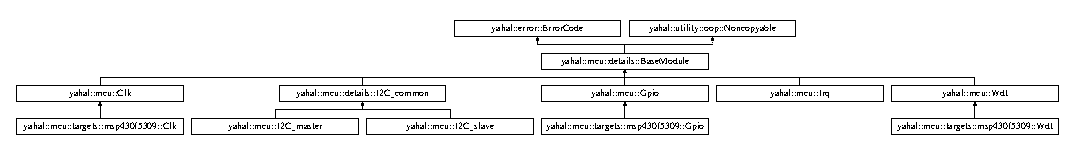
\includegraphics[height=1.575246cm]{classyahal_1_1mcu_1_1details_1_1_base_module}
\end{center}
\end{figure}
\subsection*{Public Member Functions}
\begin{DoxyCompactItemize}
\item 
bool \hyperlink{classyahal_1_1mcu_1_1details_1_1_base_module_a2389e2ad5dd20fb4cd7076dfe2f403ec}{init} (void)
\begin{DoxyCompactList}\small\item\em Public initialization method. \end{DoxyCompactList}\end{DoxyCompactItemize}
\subsection*{Protected Member Functions}
\begin{DoxyCompactItemize}
\item 
\hypertarget{classyahal_1_1mcu_1_1details_1_1_base_module_a0237a22e9f1662107cdfa4ec252e46c0}{}void \hyperlink{classyahal_1_1mcu_1_1details_1_1_base_module_a0237a22e9f1662107cdfa4ec252e46c0}{open} (void)\label{classyahal_1_1mcu_1_1details_1_1_base_module_a0237a22e9f1662107cdfa4ec252e46c0}

\begin{DoxyCompactList}\small\item\em Prepare module for exclusive operation. \end{DoxyCompactList}\item 
\hypertarget{classyahal_1_1mcu_1_1details_1_1_base_module_aa28ac444ca2c3194b30038b33da39cd7}{}void \hyperlink{classyahal_1_1mcu_1_1details_1_1_base_module_aa28ac444ca2c3194b30038b33da39cd7}{close} (void)\label{classyahal_1_1mcu_1_1details_1_1_base_module_aa28ac444ca2c3194b30038b33da39cd7}

\begin{DoxyCompactList}\small\item\em Releases module. \end{DoxyCompactList}\item 
\hypertarget{classyahal_1_1mcu_1_1details_1_1_base_module_ab4333f0c7df8ae0bcf114fa206380ca5}{}virtual void \hyperlink{classyahal_1_1mcu_1_1details_1_1_base_module_ab4333f0c7df8ae0bcf114fa206380ca5}{do\+Init} (void)=0\label{classyahal_1_1mcu_1_1details_1_1_base_module_ab4333f0c7df8ae0bcf114fa206380ca5}

\begin{DoxyCompactList}\small\item\em Must be implemented by each module. \end{DoxyCompactList}\end{DoxyCompactItemize}
\subsection*{Additional Inherited Members}


\subsection{Detailed Description}
Base class for all M\+C\+U modules. 

This class implements all methods that are common to all modules. It also inherits from noncopyable, prohibiting the copy of any class, as they are asociated to physical resources. 

Definition at line 54 of file base\+\_\+module.\+hpp.



\subsection{Member Function Documentation}
\hypertarget{classyahal_1_1mcu_1_1details_1_1_base_module_a2389e2ad5dd20fb4cd7076dfe2f403ec}{}\index{yahal\+::mcu\+::details\+::\+Base\+Module@{yahal\+::mcu\+::details\+::\+Base\+Module}!init@{init}}
\index{init@{init}!yahal\+::mcu\+::details\+::\+Base\+Module@{yahal\+::mcu\+::details\+::\+Base\+Module}}
\subsubsection[{init(void)}]{\setlength{\rightskip}{0pt plus 5cm}bool yahal\+::mcu\+::details\+::\+Base\+Module\+::init (
\begin{DoxyParamCaption}
\item[{void}]{}
\end{DoxyParamCaption}
)\hspace{0.3cm}{\ttfamily [inline]}}\label{classyahal_1_1mcu_1_1details_1_1_base_module_a2389e2ad5dd20fb4cd7076dfe2f403ec}


Public initialization method. 

It calls do\+Init. \begin{DoxySeeAlso}{See also}
\hyperlink{classyahal_1_1mcu_1_1details_1_1_base_module_ab4333f0c7df8ae0bcf114fa206380ca5}{do\+Init()} 
\end{DoxySeeAlso}


Definition at line 70 of file base\+\_\+module.\+hpp.



The documentation for this class was generated from the following file\+:\begin{DoxyCompactItemize}
\item 
/home/andy/\+Documentos/\+Source/yahal/mcu/modules/base\+\_\+module.\+hpp\end{DoxyCompactItemize}

\hypertarget{classhal_1_1battery_1_1_bq24193}{}\section{hal\+:\+:battery\+:\+:Bq24193 Class Reference}
\label{classhal_1_1battery_1_1_bq24193}\index{hal\+::battery\+::\+Bq24193@{hal\+::battery\+::\+Bq24193}}


M\+M\+M\+M\+M\+M\+M\+M\+M\+M\+M\+M\+M\+M\+M\+M\+M\+M\+M\+M\+M\+M\+M\+M\+M\+M\+M\+M\+M\+M\+M\+M\+M\+M\+M\+M\+M\+M\+M\+M\+M\+M\+M\+M\+M\+M\+M\+M\+M\+M\+M\+M\+M\+M\+M\+M\+M\+M\+M\+M\+M\+M\+M\+M\+M\+M\+M\+M\+M\+M\+M\+M\+M\+M\+M\+M\+M\+M\+M\+M\+M\+M\+M\+M\+M\+M\+M\+M\+M\+M\+M\+M\+M\+M\+M\+M\+M G\+P\+I\+O W\+W\+W\+W\+W\+W\+W\+W\+W\+W\+W\+W\+W\+W\+W\+W\+W\+W\+W\+W\+W\+W\+W\+W\+W\+W\+W\+W\+W\+W\+W\+W\+W\+W\+W\+W\+W\+W\+W\+W\+W\+W\+W\+W\+W\+W\+W\+W\+W\+W\+W\+W\+W\+W\+W\+W\+W\+W\+W\+W\+W\+W\+W\+W\+W\+W\+W\+W\+W\+W\+W\+W\+W\+W\+W\+W\+W\+W\+W\+W\+W\+W\+W\+W\+W\+W\+W\+W\+W\+W\+W\+W\+W\+W\+W\+W.  




{\ttfamily \#include $<$bq24193.\+hpp$>$}

\subsection*{Classes}
\begin{DoxyCompactItemize}
\item 
struct \hyperlink{structhal_1_1battery_1_1_bq24193_1_1_d_a_t_a___r_a_t_e}{D\+A\+T\+A\+\_\+\+R\+A\+T\+E}
\end{DoxyCompactItemize}
\subsection*{Public Member Functions}
\begin{DoxyCompactItemize}
\item 
\hypertarget{classhal_1_1battery_1_1_bq24193_ae67ceabf3e8432f9da5e7b3aa1d2b092}{}{\bfseries Bq24193} (mcu\+::\+I2\+C\+\_\+master \&i2c)\label{classhal_1_1battery_1_1_bq24193_ae67ceabf3e8432f9da5e7b3aa1d2b092}

\end{DoxyCompactItemize}
\subsection*{Public Attributes}
\begin{DoxyCompactItemize}
\item 
\hypertarget{classhal_1_1battery_1_1_bq24193_a6e195436764831719658d5efd108efd7}{}mcu\+::\+I2\+C\+\_\+master \& {\bfseries \+\_\+i2c}\label{classhal_1_1battery_1_1_bq24193_a6e195436764831719658d5efd108efd7}

\end{DoxyCompactItemize}


\subsection{Detailed Description}
M\+M\+M\+M\+M\+M\+M\+M\+M\+M\+M\+M\+M\+M\+M\+M\+M\+M\+M\+M\+M\+M\+M\+M\+M\+M\+M\+M\+M\+M\+M\+M\+M\+M\+M\+M\+M\+M\+M\+M\+M\+M\+M\+M\+M\+M\+M\+M\+M\+M\+M\+M\+M\+M\+M\+M\+M\+M\+M\+M\+M\+M\+M\+M\+M\+M\+M\+M\+M\+M\+M\+M\+M\+M\+M\+M\+M\+M\+M\+M\+M\+M\+M\+M\+M\+M\+M\+M\+M\+M\+M\+M\+M\+M\+M\+M\+M G\+P\+I\+O W\+W\+W\+W\+W\+W\+W\+W\+W\+W\+W\+W\+W\+W\+W\+W\+W\+W\+W\+W\+W\+W\+W\+W\+W\+W\+W\+W\+W\+W\+W\+W\+W\+W\+W\+W\+W\+W\+W\+W\+W\+W\+W\+W\+W\+W\+W\+W\+W\+W\+W\+W\+W\+W\+W\+W\+W\+W\+W\+W\+W\+W\+W\+W\+W\+W\+W\+W\+W\+W\+W\+W\+W\+W\+W\+W\+W\+W\+W\+W\+W\+W\+W\+W\+W\+W\+W\+W\+W\+W\+W\+W\+W\+W\+W\+W. 

Definition at line 57 of file bq24193.\+hpp.



The documentation for this class was generated from the following file\+:\begin{DoxyCompactItemize}
\item 
/home/andy/\+Documentos/\+Source/yahal/sensors/bq24193/bq24193.\+hpp\end{DoxyCompactItemize}

\hypertarget{classyahal_1_1utility_1_1oop_1_1_callback}{}\section{yahal\+:\+:utility\+:\+:oop\+:\+:Callback$<$ T\+\_\+\+A\+R\+G\+U\+M\+E\+N\+T $>$ Class Template Reference}
\label{classyahal_1_1utility_1_1oop_1_1_callback}\index{yahal\+::utility\+::oop\+::\+Callback$<$ T\+\_\+\+A\+R\+G\+U\+M\+E\+N\+T $>$@{yahal\+::utility\+::oop\+::\+Callback$<$ T\+\_\+\+A\+R\+G\+U\+M\+E\+N\+T $>$}}


============================================================================== W\+I\+T\+H A\+R\+G\+U\+M\+E\+N\+T  




{\ttfamily \#include $<$callback.\+hpp$>$}

\subsection*{Public Member Functions}
\begin{DoxyCompactItemize}
\item 
\hypertarget{classyahal_1_1utility_1_1oop_1_1_callback_a98bf2f87baa4b37ca913d87b299739fd}{}void {\bfseries set\+Call\+Back\+Function} (void($\ast$fp\+Call\+On\+Trigger)(T\+\_\+\+A\+R\+G\+U\+M\+E\+N\+T))\label{classyahal_1_1utility_1_1oop_1_1_callback_a98bf2f87baa4b37ca913d87b299739fd}

\item 
\hypertarget{classyahal_1_1utility_1_1oop_1_1_callback_adca95cbca0615399bac9ae47b3891c96}{}bool {\bfseries run} (T\+\_\+\+A\+R\+G\+U\+M\+E\+N\+T argument) const \label{classyahal_1_1utility_1_1oop_1_1_callback_adca95cbca0615399bac9ae47b3891c96}

\end{DoxyCompactItemize}


\subsection{Detailed Description}
\subsubsection*{template$<$typename T\+\_\+\+A\+R\+G\+U\+M\+E\+N\+T$>$class yahal\+::utility\+::oop\+::\+Callback$<$ T\+\_\+\+A\+R\+G\+U\+M\+E\+N\+T $>$}

============================================================================== W\+I\+T\+H A\+R\+G\+U\+M\+E\+N\+T 

Definition at line 37 of file callback.\+hpp.



The documentation for this class was generated from the following file\+:\begin{DoxyCompactItemize}
\item 
/home/andy/\+Documentos/\+Source/yahal/utility/oop/callback.\+hpp\end{DoxyCompactItemize}

\hypertarget{classyahal_1_1utility_1_1oop_1_1_callback_3_01void_01_4}{}\section{yahal\+:\+:utility\+:\+:oop\+:\+:Callback$<$ void $>$ Class Template Reference}
\label{classyahal_1_1utility_1_1oop_1_1_callback_3_01void_01_4}\index{yahal\+::utility\+::oop\+::\+Callback$<$ void $>$@{yahal\+::utility\+::oop\+::\+Callback$<$ void $>$}}


=========================================================================== W\+I\+T\+H\+O\+U\+T A\+R\+G\+U\+M\+E\+N\+T  




{\ttfamily \#include $<$callback.\+hpp$>$}

\subsection*{Public Member Functions}
\begin{DoxyCompactItemize}
\item 
\hypertarget{classyahal_1_1utility_1_1oop_1_1_callback_3_01void_01_4_ad2f0d55b5a796e8537e359ae766acb54}{}void {\bfseries set\+Call\+Back\+Function} (void($\ast$fp\+Call\+On\+Trigger)(void))\label{classyahal_1_1utility_1_1oop_1_1_callback_3_01void_01_4_ad2f0d55b5a796e8537e359ae766acb54}

\item 
\hypertarget{classyahal_1_1utility_1_1oop_1_1_callback_3_01void_01_4_a0d1ef309320425a2606086152b1f97fa}{}bool {\bfseries run} (void) const \label{classyahal_1_1utility_1_1oop_1_1_callback_3_01void_01_4_a0d1ef309320425a2606086152b1f97fa}

\end{DoxyCompactItemize}


\subsection{Detailed Description}
\subsubsection*{template$<$$>$class yahal\+::utility\+::oop\+::\+Callback$<$ void $>$}

=========================================================================== W\+I\+T\+H\+O\+U\+T A\+R\+G\+U\+M\+E\+N\+T 

Definition at line 81 of file callback.\+hpp.



The documentation for this class was generated from the following file\+:\begin{DoxyCompactItemize}
\item 
/home/andy/\+Documentos/\+Source/yahal/utility/oop/callback.\+hpp\end{DoxyCompactItemize}

\hypertarget{classyahal_1_1mcu_1_1targets_1_1msp430f5309_1_1_clk}{}\section{yahal\+:\+:mcu\+:\+:targets\+:\+:msp430f5309\+:\+:Clk Class Reference}
\label{classyahal_1_1mcu_1_1targets_1_1msp430f5309_1_1_clk}\index{yahal\+::mcu\+::targets\+::msp430f5309\+::\+Clk@{yahal\+::mcu\+::targets\+::msp430f5309\+::\+Clk}}


\begin{DoxyVerb}\end{DoxyVerb}
  




{\ttfamily \#include $<$clk.\+hpp$>$}

Inheritance diagram for yahal\+:\+:mcu\+:\+:targets\+:\+:msp430f5309\+:\+:Clk\+:\begin{figure}[H]
\begin{center}
\leavevmode
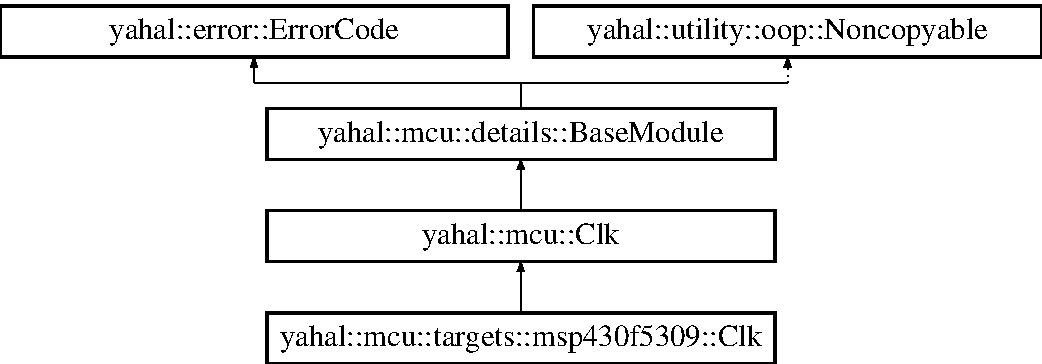
\includegraphics[height=4.000000cm]{classyahal_1_1mcu_1_1targets_1_1msp430f5309_1_1_clk}
\end{center}
\end{figure}
\subsection*{Classes}
\begin{DoxyCompactItemize}
\item 
struct \hyperlink{structyahal_1_1mcu_1_1targets_1_1msp430f5309_1_1_clk_1_1_frequency}{Frequency}
\end{DoxyCompactItemize}
\subsection*{Additional Inherited Members}


\subsection{Detailed Description}
\begin{DoxyVerb}\end{DoxyVerb}
 

Definition at line 50 of file clk.\+hpp.



The documentation for this class was generated from the following files\+:\begin{DoxyCompactItemize}
\item 
/home/andy/\+Documentos/\+Source/yahal/mcu/targets/msp430f5309/clk/clk.\+hpp\item 
/home/andy/\+Documentos/\+Source/yahal/mcu/targets/msp430f5309/clk/clk.\+cpp\end{DoxyCompactItemize}

\hypertarget{classyahal_1_1mcu_1_1_clk}{}\section{yahal\+:\+:mcu\+:\+:Clk Class Reference}
\label{classyahal_1_1mcu_1_1_clk}\index{yahal\+::mcu\+::\+Clk@{yahal\+::mcu\+::\+Clk}}


Base class for all system clock handling modules.  




{\ttfamily \#include $<$clk.\+hpp$>$}

Inheritance diagram for yahal\+:\+:mcu\+:\+:Clk\+:\begin{figure}[H]
\begin{center}
\leavevmode
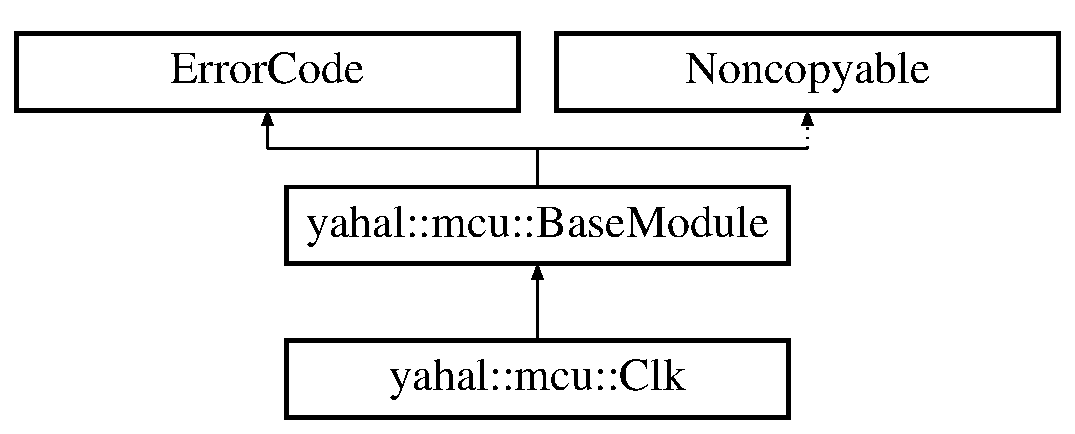
\includegraphics[height=4.000000cm]{classyahal_1_1mcu_1_1_clk}
\end{center}
\end{figure}
\subsection*{Classes}
\begin{DoxyCompactItemize}
\item 
struct \hyperlink{structyahal_1_1mcu_1_1_clk_1_1_error}{Error}
\end{DoxyCompactItemize}
\subsection*{Additional Inherited Members}


\subsection{Detailed Description}
Base class for all system clock handling modules. 

Definition at line 47 of file clk.\+hpp.



The documentation for this class was generated from the following file\+:\begin{DoxyCompactItemize}
\item 
/home/andy/\+Documentos/\+Source/yahal/mcu/modules/clk/clk.\+hpp\end{DoxyCompactItemize}

\hypertarget{classhal_1_1utility_1_1_counter}{}\section{hal\+:\+:utility\+:\+:Counter$<$ T $>$ Class Template Reference}
\label{classhal_1_1utility_1_1_counter}\index{hal\+::utility\+::\+Counter$<$ T $>$@{hal\+::utility\+::\+Counter$<$ T $>$}}


\subsection{Detailed Description}
\subsubsection*{template$<$typename T$>$class hal\+::utility\+::\+Counter$<$ T $>$}



Definition at line 41 of file counter.\+hpp.



The documentation for this class was generated from the following file\+:\begin{DoxyCompactItemize}
\item 
/home/andy/\+Documentos/\+Source/yahal/utility/counter.\+hpp\end{DoxyCompactItemize}

\hypertarget{structhal_1_1sensors_1_1_ads1115_1_1_d_a_t_a___r_a_t_e}{}\section{hal\+:\+:sensors\+:\+:Ads1115\+:\+:D\+A\+T\+A\+\_\+\+R\+A\+T\+E Struct Reference}
\label{structhal_1_1sensors_1_1_ads1115_1_1_d_a_t_a___r_a_t_e}\index{hal\+::sensors\+::\+Ads1115\+::\+D\+A\+T\+A\+\_\+\+R\+A\+T\+E@{hal\+::sensors\+::\+Ads1115\+::\+D\+A\+T\+A\+\_\+\+R\+A\+T\+E}}
\subsection*{Public Types}
\begin{DoxyCompactItemize}
\item 
\hypertarget{structhal_1_1sensors_1_1_ads1115_1_1_d_a_t_a___r_a_t_e_a85e533bbdebc2ef3ab4a55e83c4b3128}{}enum {\bfseries type} \{ \\*
{\bfseries S\+P\+S\+\_\+8} = 0b000, 
{\bfseries S\+P\+S\+\_\+16} = 0b001, 
{\bfseries S\+P\+S\+\_\+32} = 0b010, 
{\bfseries S\+P\+S\+\_\+64} = 0b011, 
\\*
{\bfseries S\+P\+S\+\_\+128} = 0b100, 
{\bfseries S\+P\+S\+\_\+250} = 0b101, 
{\bfseries S\+P\+S\+\_\+475} = 0b110, 
{\bfseries S\+P\+S\+\_\+860} = 0b111
 \}\label{structhal_1_1sensors_1_1_ads1115_1_1_d_a_t_a___r_a_t_e_a85e533bbdebc2ef3ab4a55e83c4b3128}

\end{DoxyCompactItemize}


\subsection{Detailed Description}


Definition at line 60 of file ads1115.\+hpp.



The documentation for this struct was generated from the following file\+:\begin{DoxyCompactItemize}
\item 
/home/andy/\+Documentos/\+Source/yahal/sensors/ads1115/ads1115.\+hpp\end{DoxyCompactItemize}

\hypertarget{structhal_1_1battery_1_1_bq24193_1_1_d_a_t_a___r_a_t_e}{}\section{hal\+:\+:battery\+:\+:Bq24193\+:\+:D\+A\+T\+A\+\_\+\+R\+A\+T\+E Struct Reference}
\label{structhal_1_1battery_1_1_bq24193_1_1_d_a_t_a___r_a_t_e}\index{hal\+::battery\+::\+Bq24193\+::\+D\+A\+T\+A\+\_\+\+R\+A\+T\+E@{hal\+::battery\+::\+Bq24193\+::\+D\+A\+T\+A\+\_\+\+R\+A\+T\+E}}
\subsection*{Public Types}
\begin{DoxyCompactItemize}
\item 
\hypertarget{structhal_1_1battery_1_1_bq24193_1_1_d_a_t_a___r_a_t_e_ad312cb38ca9fc66e0f669d12721568ea}{}enum {\bfseries type} \label{structhal_1_1battery_1_1_bq24193_1_1_d_a_t_a___r_a_t_e_ad312cb38ca9fc66e0f669d12721568ea}

\end{DoxyCompactItemize}


\subsection{Detailed Description}


Definition at line 60 of file bq24193.\+hpp.



The documentation for this struct was generated from the following file\+:\begin{DoxyCompactItemize}
\item 
/home/andy/\+Documentos/\+Source/yahal/sensors/bq24193/bq24193.\+hpp\end{DoxyCompactItemize}

\hypertarget{structyahal_1_1mcu_1_1_gpio_1_1_direction}{}\section{yahal\+:\+:mcu\+:\+:Gpio\+:\+:Direction Struct Reference}
\label{structyahal_1_1mcu_1_1_gpio_1_1_direction}\index{yahal\+::mcu\+::\+Gpio\+::\+Direction@{yahal\+::mcu\+::\+Gpio\+::\+Direction}}


\hyperlink{structyahal_1_1mcu_1_1_gpio_1_1_direction}{Direction} of G\+P\+I\+O pins.  




{\ttfamily \#include $<$gpio.\+hpp$>$}

\subsection*{Public Types}
\begin{DoxyCompactItemize}
\item 
\hypertarget{structyahal_1_1mcu_1_1_gpio_1_1_direction_a439a47640b093599989104f4260ddea5}{}enum {\bfseries Type} \{ {\bfseries I\+N\+P\+U\+T} = false, 
{\bfseries O\+U\+T\+P\+U\+T} = true
 \}\label{structyahal_1_1mcu_1_1_gpio_1_1_direction_a439a47640b093599989104f4260ddea5}

\end{DoxyCompactItemize}


\subsection{Detailed Description}
\hyperlink{structyahal_1_1mcu_1_1_gpio_1_1_direction}{Direction} of G\+P\+I\+O pins. 

Definition at line 54 of file gpio.\+hpp.



The documentation for this struct was generated from the following file\+:\begin{DoxyCompactItemize}
\item 
/home/andy/\+Documentos/\+Source/yahal/mcu/modules/gpio/gpio.\+hpp\end{DoxyCompactItemize}

\hypertarget{structyahal_1_1mcu_1_1details_1_1_i2_c__common_1_1_direction}{}\section{yahal\+:\+:mcu\+:\+:details\+:\+:I2\+C\+\_\+common\+:\+:Direction Struct Reference}
\label{structyahal_1_1mcu_1_1details_1_1_i2_c__common_1_1_direction}\index{yahal\+::mcu\+::details\+::\+I2\+C\+\_\+common\+::\+Direction@{yahal\+::mcu\+::details\+::\+I2\+C\+\_\+common\+::\+Direction}}


I/\+O operation direction.  




{\ttfamily \#include $<$i2c\+\_\+common.\+hpp$>$}

\subsection*{Public Types}
\begin{DoxyCompactItemize}
\item 
\hypertarget{structyahal_1_1mcu_1_1details_1_1_i2_c__common_1_1_direction_a13e2000f0f779540af7efbc0f744b420}{}enum {\bfseries Type} \{ {\bfseries R\+E\+A\+D}, 
{\bfseries W\+R\+I\+T\+E}
 \}\label{structyahal_1_1mcu_1_1details_1_1_i2_c__common_1_1_direction_a13e2000f0f779540af7efbc0f744b420}

\end{DoxyCompactItemize}


\subsection{Detailed Description}
I/\+O operation direction. 

Definition at line 55 of file i2c\+\_\+common.\+hpp.



The documentation for this struct was generated from the following file\+:\begin{DoxyCompactItemize}
\item 
/home/andy/\+Documentos/\+Source/yahal/mcu/modules/i2c/i2c\+\_\+common.\+hpp\end{DoxyCompactItemize}

\hypertarget{structyahal_1_1mcu_1_1_gpio_1_1_error}{}\section{yahal\+:\+:mcu\+:\+:Gpio\+:\+:Error Struct Reference}
\label{structyahal_1_1mcu_1_1_gpio_1_1_error}\index{yahal\+::mcu\+::\+Gpio\+::\+Error@{yahal\+::mcu\+::\+Gpio\+::\+Error}}


G\+P\+I\+O errors.  




{\ttfamily \#include $<$gpio.\+hpp$>$}

\subsection*{Public Types}
\begin{DoxyCompactItemize}
\item 
\hypertarget{structyahal_1_1mcu_1_1_gpio_1_1_error_a3cdf8682538fd41409200af5008458af}{}enum {\bfseries Type} \{ \\*
{\bfseries N\+O\+\_\+\+E\+R\+R\+O\+R} = 0, 
{\bfseries T\+R\+Y\+I\+N\+G\+\_\+\+T\+O\+\_\+\+A\+C\+C\+E\+S\+S\+\_\+\+N\+O\+N\+\_\+\+E\+X\+I\+S\+T\+A\+N\+T\+\_\+\+P\+O\+R\+T}, 
{\bfseries T\+R\+Y\+I\+N\+G\+\_\+\+T\+O\+\_\+\+A\+C\+C\+E\+S\+S\+\_\+\+N\+O\+N\+\_\+\+E\+X\+I\+S\+T\+A\+N\+T\+\_\+\+P\+I\+N}, 
{\bfseries C\+O\+U\+L\+D\+\_\+\+N\+O\+T\+\_\+\+I\+N\+I\+T\+I\+A\+L\+I\+Z\+E\+\_\+\+P\+O\+R\+T}, 
\\*
{\bfseries P\+U\+L\+L\+U\+P\+\_\+\+Resistor\+\_\+\+N\+O\+T\+\_\+\+A\+V\+A\+I\+L\+A\+B\+L\+E}, 
{\bfseries P\+U\+L\+L\+D\+O\+W\+N\+\_\+\+Resistor\+\_\+\+N\+O\+T\+\_\+\+A\+V\+A\+I\+L\+A\+B\+L\+E}, 
{\bfseries O\+T\+H\+E\+R}
 \}\label{structyahal_1_1mcu_1_1_gpio_1_1_error_a3cdf8682538fd41409200af5008458af}

\end{DoxyCompactItemize}


\subsection{Detailed Description}
G\+P\+I\+O errors. 

Definition at line 72 of file gpio.\+hpp.



The documentation for this struct was generated from the following file\+:\begin{DoxyCompactItemize}
\item 
/home/andy/\+Documentos/\+Source/yahal/mcu/modules/gpio/gpio.\+hpp\end{DoxyCompactItemize}

\hypertarget{structyahal_1_1mcu_1_1_clk_1_1_error}{}\section{yahal\+:\+:mcu\+:\+:Clk\+:\+:Error Struct Reference}
\label{structyahal_1_1mcu_1_1_clk_1_1_error}\index{yahal\+::mcu\+::\+Clk\+::\+Error@{yahal\+::mcu\+::\+Clk\+::\+Error}}
\subsection*{Public Types}
\begin{DoxyCompactItemize}
\item 
\hypertarget{structyahal_1_1mcu_1_1_clk_1_1_error_a2adeac4ff415df9b1cfe8707f88ae2ab}{}enum {\bfseries Type} \{ {\bfseries N\+O\+\_\+\+E\+R\+R\+O\+R} = N\+O\+\_\+\+E\+R\+R\+O\+R\+\_\+\+C\+O\+D\+E, 
{\bfseries F\+R\+E\+Q\+U\+E\+N\+C\+Y\+\_\+\+N\+O\+T\+\_\+\+A\+V\+A\+I\+L\+A\+B\+L\+E}, 
{\bfseries O\+T\+H\+E\+R}
 \}\label{structyahal_1_1mcu_1_1_clk_1_1_error_a2adeac4ff415df9b1cfe8707f88ae2ab}

\end{DoxyCompactItemize}


\subsection{Detailed Description}


Definition at line 50 of file clk.\+hpp.



The documentation for this struct was generated from the following file\+:\begin{DoxyCompactItemize}
\item 
/home/andy/\+Documentos/\+Source/yahal/mcu/modules/clk/clk.\+hpp\end{DoxyCompactItemize}

\hypertarget{structyahal_1_1mcu_1_1_irq_1_1_error}{}\section{yahal\+:\+:mcu\+:\+:Irq\+:\+:Error Struct Reference}
\label{structyahal_1_1mcu_1_1_irq_1_1_error}\index{yahal\+::mcu\+::\+Irq\+::\+Error@{yahal\+::mcu\+::\+Irq\+::\+Error}}
\subsection*{Public Types}
\begin{DoxyCompactItemize}
\item 
\hypertarget{structyahal_1_1mcu_1_1_irq_1_1_error_a8c9fff4148f08531ba5cbfe02f60f63d}{}enum {\bfseries Type} \{ {\bfseries N\+O\+\_\+\+E\+R\+R\+O\+R} = 0, 
{\bfseries O\+T\+H\+E\+R}
 \}\label{structyahal_1_1mcu_1_1_irq_1_1_error_a8c9fff4148f08531ba5cbfe02f60f63d}

\end{DoxyCompactItemize}


\subsection{Detailed Description}


Definition at line 87 of file irq.\+hpp.



The documentation for this struct was generated from the following file\+:\begin{DoxyCompactItemize}
\item 
/home/andy/\+Documentos/\+Source/yahal/mcu/modules/irq/irq.\+hpp\end{DoxyCompactItemize}

\hypertarget{structyahal_1_1mcu_1_1_wdt_1_1_error}{}\section{yahal\+:\+:mcu\+:\+:Wdt\+:\+:Error Struct Reference}
\label{structyahal_1_1mcu_1_1_wdt_1_1_error}\index{yahal\+::mcu\+::\+Wdt\+::\+Error@{yahal\+::mcu\+::\+Wdt\+::\+Error}}
\subsection*{Public Types}
\begin{DoxyCompactItemize}
\item 
\hypertarget{structyahal_1_1mcu_1_1_wdt_1_1_error_aca128594025d015df655e4e9c311e5b2}{}enum {\bfseries Type} \{ {\bfseries N\+O\+\_\+\+E\+R\+R\+O\+R} = 0, 
{\bfseries O\+T\+H\+E\+R}
 \}\label{structyahal_1_1mcu_1_1_wdt_1_1_error_aca128594025d015df655e4e9c311e5b2}

\end{DoxyCompactItemize}


\subsection{Detailed Description}


Definition at line 52 of file wdt.\+hpp.



The documentation for this struct was generated from the following file\+:\begin{DoxyCompactItemize}
\item 
/home/andy/\+Documentos/\+Source/yahal/mcu/modules/wdt/wdt.\+hpp\end{DoxyCompactItemize}

\hypertarget{structyahal_1_1mcu_1_1details_1_1_i2_c__common_1_1_error}{}\section{yahal\+:\+:mcu\+:\+:details\+:\+:I2\+C\+\_\+common\+:\+:Error Struct Reference}
\label{structyahal_1_1mcu_1_1details_1_1_i2_c__common_1_1_error}\index{yahal\+::mcu\+::details\+::\+I2\+C\+\_\+common\+::\+Error@{yahal\+::mcu\+::details\+::\+I2\+C\+\_\+common\+::\+Error}}


\hyperlink{structyahal_1_1mcu_1_1details_1_1_i2_c__common_1_1_error}{Error} codes for I2\+C.  




{\ttfamily \#include $<$i2c\+\_\+common.\+hpp$>$}

\subsection*{Public Types}
\begin{DoxyCompactItemize}
\item 
\hypertarget{structyahal_1_1mcu_1_1details_1_1_i2_c__common_1_1_error_a8b8e77837be54467fe7bc9ecb823453b}{}enum {\bfseries Type} \{ \\*
{\bfseries N\+O\+\_\+\+E\+R\+R\+O\+R} = N\+O\+\_\+\+E\+R\+R\+O\+R\+\_\+\+C\+O\+D\+E, 
{\bfseries S\+L\+A\+V\+E\+\_\+\+A\+D\+D\+R\+E\+S\+S\+\_\+\+N\+O\+T\+\_\+7\+\_\+\+B\+I\+T}, 
{\bfseries S\+L\+A\+V\+E\+\_\+\+N\+O\+T\+\_\+\+R\+E\+A\+C\+H\+A\+B\+L\+E}, 
{\bfseries S\+L\+A\+V\+E\+\_\+\+D\+A\+T\+A\+\_\+\+N\+A\+C\+K}, 
\\*
{\bfseries I\+N\+V\+A\+L\+I\+D\+\_\+\+M\+E\+S\+S\+A\+G\+E\+\_\+\+B\+U\+F\+F\+E\+R}, 
{\bfseries R\+E\+A\+D\+\_\+\+O\+V\+E\+R\+F\+L\+O\+W\+\_\+\+A\+T\+T\+E\+M\+P\+T}, 
{\bfseries Z\+E\+R\+O\+\_\+\+S\+I\+Z\+E\+\_\+\+M\+E\+S\+S\+A\+G\+E}, 
{\bfseries T\+R\+A\+N\+S\+M\+I\+S\+S\+I\+O\+N\+\_\+\+P\+R\+E\+M\+A\+T\+U\+R\+E\+L\+Y\+\_\+\+E\+N\+D\+E\+D}
 \}\label{structyahal_1_1mcu_1_1details_1_1_i2_c__common_1_1_error_a8b8e77837be54467fe7bc9ecb823453b}

\end{DoxyCompactItemize}


\subsection{Detailed Description}
\hyperlink{structyahal_1_1mcu_1_1details_1_1_i2_c__common_1_1_error}{Error} codes for I2\+C. 

Definition at line 66 of file i2c\+\_\+common.\+hpp.



The documentation for this struct was generated from the following file\+:\begin{DoxyCompactItemize}
\item 
/home/andy/\+Documentos/\+Source/yahal/mcu/modules/i2c/i2c\+\_\+common.\+hpp\end{DoxyCompactItemize}

\hypertarget{classyahal_1_1error_1_1_error_code}{}\section{yahal\+:\+:error\+:\+:Error\+Code Class Reference}
\label{classyahal_1_1error_1_1_error_code}\index{yahal\+::error\+::\+Error\+Code@{yahal\+::error\+::\+Error\+Code}}


Error code.  




{\ttfamily \#include $<$error\+\_\+code.\+hpp$>$}

Inheritance diagram for yahal\+:\+:error\+:\+:Error\+Code\+:\begin{figure}[H]
\begin{center}
\leavevmode
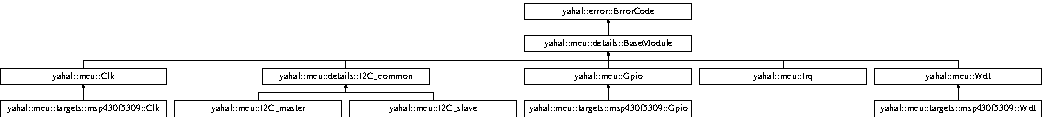
\includegraphics[height=3.000000cm]{classyahal_1_1error_1_1_error_code}
\end{center}
\end{figure}
\subsection*{Public Member Functions}
\begin{DoxyCompactItemize}
\item 
\hypertarget{classyahal_1_1error_1_1_error_code_a8da8151a2788d474084d789337d97bae}{}unsigned int {\bfseries get\+Error\+Code} (void) const \label{classyahal_1_1error_1_1_error_code_a8da8151a2788d474084d789337d97bae}

\item 
\hypertarget{classyahal_1_1error_1_1_error_code_a2c92ad4dd5a16cd0f994fb14d35f2245}{}bool {\bfseries has\+Error} (void) const \label{classyahal_1_1error_1_1_error_code_a2c92ad4dd5a16cd0f994fb14d35f2245}

\end{DoxyCompactItemize}
\subsection*{Protected Member Functions}
\begin{DoxyCompactItemize}
\item 
void \hyperlink{classyahal_1_1error_1_1_error_code_acc2142f7c7fad8b06e9933611e8a5a31}{set\+Error\+Code} (unsigned int new\+Error\+Code)
\begin{DoxyCompactList}\small\item\em Set new error code. \end{DoxyCompactList}\item 
void \hyperlink{classyahal_1_1error_1_1_error_code_a6dcccae993641509661b2f92c702b714}{clear\+Error\+Code} (void)
\begin{DoxyCompactList}\small\item\em Clear error code. \end{DoxyCompactList}\end{DoxyCompactItemize}
\subsection*{Static Protected Attributes}
\begin{DoxyCompactItemize}
\item 
\hypertarget{classyahal_1_1error_1_1_error_code_a190aff352d405f5859ed2134017643d4}{}static const unsigned int {\bfseries N\+O\+\_\+\+E\+R\+R\+O\+R} = 0\label{classyahal_1_1error_1_1_error_code_a190aff352d405f5859ed2134017643d4}

\end{DoxyCompactItemize}


\subsection{Detailed Description}
Error code. 

Definition at line 48 of file error\+\_\+code.\+hpp.



\subsection{Member Function Documentation}
\hypertarget{classyahal_1_1error_1_1_error_code_a6dcccae993641509661b2f92c702b714}{}\index{yahal\+::error\+::\+Error\+Code@{yahal\+::error\+::\+Error\+Code}!clear\+Error\+Code@{clear\+Error\+Code}}
\index{clear\+Error\+Code@{clear\+Error\+Code}!yahal\+::error\+::\+Error\+Code@{yahal\+::error\+::\+Error\+Code}}
\subsubsection[{clear\+Error\+Code(void)}]{\setlength{\rightskip}{0pt plus 5cm}void yahal\+::error\+::\+Error\+Code\+::clear\+Error\+Code (
\begin{DoxyParamCaption}
\item[{void}]{}
\end{DoxyParamCaption}
)\hspace{0.3cm}{\ttfamily [inline]}, {\ttfamily [protected]}}\label{classyahal_1_1error_1_1_error_code_a6dcccae993641509661b2f92c702b714}


Clear error code. 

Identical to \char`\"{}set\+Error\+Code(\+N\+O\+\_\+\+E\+R\+R\+O\+R)\char`\"{}. \begin{DoxySeeAlso}{See also}
\hyperlink{classyahal_1_1error_1_1_error_code_acc2142f7c7fad8b06e9933611e8a5a31}{set\+Error\+Code}. 
\end{DoxySeeAlso}


Definition at line 98 of file error\+\_\+code.\+hpp.

\hypertarget{classyahal_1_1error_1_1_error_code_acc2142f7c7fad8b06e9933611e8a5a31}{}\index{yahal\+::error\+::\+Error\+Code@{yahal\+::error\+::\+Error\+Code}!set\+Error\+Code@{set\+Error\+Code}}
\index{set\+Error\+Code@{set\+Error\+Code}!yahal\+::error\+::\+Error\+Code@{yahal\+::error\+::\+Error\+Code}}
\subsubsection[{set\+Error\+Code(unsigned int new\+Error\+Code)}]{\setlength{\rightskip}{0pt plus 5cm}void yahal\+::error\+::\+Error\+Code\+::set\+Error\+Code (
\begin{DoxyParamCaption}
\item[{unsigned int}]{new\+Error\+Code}
\end{DoxyParamCaption}
)\hspace{0.3cm}{\ttfamily [inline]}, {\ttfamily [protected]}}\label{classyahal_1_1error_1_1_error_code_acc2142f7c7fad8b06e9933611e8a5a31}


Set new error code. 

Allows derived classes to set a new error code. 

Definition at line 86 of file error\+\_\+code.\+hpp.



The documentation for this class was generated from the following file\+:\begin{DoxyCompactItemize}
\item 
/home/andy/\+Documentos/\+Source/yahal/error/error\+\_\+code.\+hpp\end{DoxyCompactItemize}

\hypertarget{structyahal_1_1mcu_1_1targets_1_1msp430f5309_1_1_clk_1_1_frequency}{}\section{yahal\+:\+:mcu\+:\+:targets\+:\+:msp430f5309\+:\+:Clk\+:\+:Frequency Struct Reference}
\label{structyahal_1_1mcu_1_1targets_1_1msp430f5309_1_1_clk_1_1_frequency}\index{yahal\+::mcu\+::targets\+::msp430f5309\+::\+Clk\+::\+Frequency@{yahal\+::mcu\+::targets\+::msp430f5309\+::\+Clk\+::\+Frequency}}
\subsection*{Public Types}
\begin{DoxyCompactItemize}
\item 
\hypertarget{structyahal_1_1mcu_1_1targets_1_1msp430f5309_1_1_clk_1_1_frequency_a32962c9ff596c457b230044a7f209b26}{}enum {\bfseries Type} \{ \\*
{\bfseries D\+C\+O\+\_\+1\+M\+Hz} = 1000000, 
{\bfseries D\+C\+O\+\_\+2\+M\+Hz} = 2000000, 
{\bfseries D\+C\+O\+\_\+4\+M\+Hz} = 4000000, 
{\bfseries D\+C\+O\+\_\+8\+M\+Hz} = 8000000, 
\\*
{\bfseries D\+C\+O\+\_\+16\+M\+Hz} = 16000000, 
{\bfseries D\+C\+O\+\_\+32\+M\+Hz} = 32000000
 \}\label{structyahal_1_1mcu_1_1targets_1_1msp430f5309_1_1_clk_1_1_frequency_a32962c9ff596c457b230044a7f209b26}

\end{DoxyCompactItemize}


\subsection{Detailed Description}


Definition at line 53 of file clk.\+hpp.



The documentation for this struct was generated from the following file\+:\begin{DoxyCompactItemize}
\item 
/home/andy/\+Documentos/\+Source/yahal/mcu/targets/msp430f5309/clk/clk.\+hpp\end{DoxyCompactItemize}

\hypertarget{classyahal_1_1mcu_1_1targets_1_1msp430f5309_1_1_gpio}{}\section{yahal\+:\+:mcu\+:\+:targets\+:\+:msp430f5309\+:\+:Gpio Class Reference}
\label{classyahal_1_1mcu_1_1targets_1_1msp430f5309_1_1_gpio}\index{yahal\+::mcu\+::targets\+::msp430f5309\+::\+Gpio@{yahal\+::mcu\+::targets\+::msp430f5309\+::\+Gpio}}


\begin{DoxyVerb}\end{DoxyVerb}
  




{\ttfamily \#include $<$gpio.\+hpp$>$}

Inheritance diagram for yahal\+:\+:mcu\+:\+:targets\+:\+:msp430f5309\+:\+:Gpio\+:\begin{figure}[H]
\begin{center}
\leavevmode
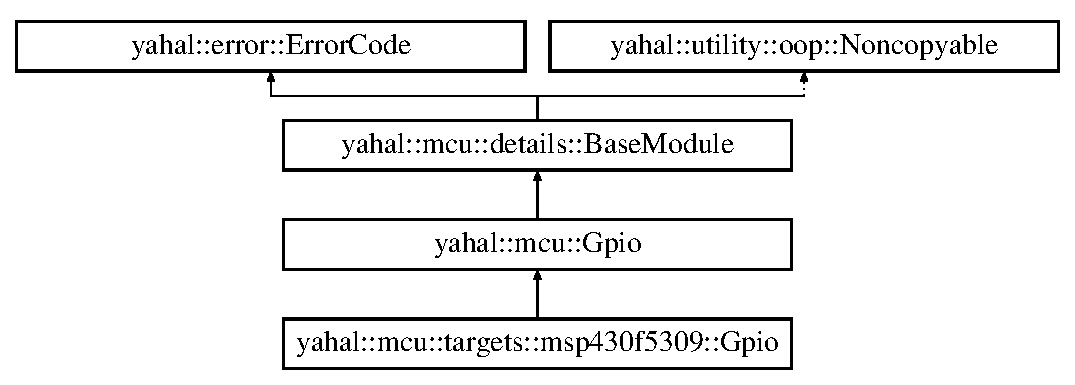
\includegraphics[height=4.000000cm]{classyahal_1_1mcu_1_1targets_1_1msp430f5309_1_1_gpio}
\end{center}
\end{figure}
\subsection*{Public Member Functions}
\begin{DoxyCompactItemize}
\item 
\hypertarget{classyahal_1_1mcu_1_1targets_1_1msp430f5309_1_1_gpio_a0a1b6223b22432357fbca9fe1732ed9c}{}\hyperlink{classyahal_1_1mcu_1_1_gpio_1_1_port}{yahal\+::mcu\+::\+Gpio\+::\+Port} \& \hyperlink{classyahal_1_1mcu_1_1targets_1_1msp430f5309_1_1_gpio_a0a1b6223b22432357fbca9fe1732ed9c}{port} (uint8\+\_\+t port\+Number)\label{classyahal_1_1mcu_1_1targets_1_1msp430f5309_1_1_gpio_a0a1b6223b22432357fbca9fe1732ed9c}

\begin{DoxyCompactList}\small\item\em Return reference to port. \end{DoxyCompactList}\end{DoxyCompactItemize}
\subsection*{Additional Inherited Members}


\subsection{Detailed Description}
\begin{DoxyVerb}\end{DoxyVerb}
 

Definition at line 50 of file gpio.\+hpp.



The documentation for this class was generated from the following files\+:\begin{DoxyCompactItemize}
\item 
/home/andy/\+Documentos/\+Source/yahal/mcu/targets/msp430f5309/gpio/gpio.\+hpp\item 
/home/andy/\+Documentos/\+Source/yahal/mcu/targets/msp430f5309/gpio/gpio.\+cpp\end{DoxyCompactItemize}

\hypertarget{structyahal_1_1mcu_1_1_irq_1_1_g_p_i_o}{}\section{yahal\+:\+:mcu\+:\+:Irq\+:\+:G\+P\+I\+O Struct Reference}
\label{structyahal_1_1mcu_1_1_irq_1_1_g_p_i_o}\index{yahal\+::mcu\+::\+Irq\+::\+G\+P\+I\+O@{yahal\+::mcu\+::\+Irq\+::\+G\+P\+I\+O}}
\subsection*{Public Types}
\begin{DoxyCompactItemize}
\item 
\hypertarget{structyahal_1_1mcu_1_1_irq_1_1_g_p_i_o_a32d7b87ae60ee74fae28b3df5ff17d1f}{}enum {\bfseries type} \{ {\bfseries A}, 
{\bfseries B}
 \}\label{structyahal_1_1mcu_1_1_irq_1_1_g_p_i_o_a32d7b87ae60ee74fae28b3df5ff17d1f}

\end{DoxyCompactItemize}


\subsection{Detailed Description}


Definition at line 79 of file irq.\+hpp.



The documentation for this struct was generated from the following file\+:\begin{DoxyCompactItemize}
\item 
/home/andy/\+Documentos/\+Source/yahal/mcu/modules/irq/irq.\+hpp\end{DoxyCompactItemize}

\hypertarget{classyahal_1_1mcu_1_1_gpio}{}\section{yahal\+:\+:mcu\+:\+:Gpio Class Reference}
\label{classyahal_1_1mcu_1_1_gpio}\index{yahal\+::mcu\+::\+Gpio@{yahal\+::mcu\+::\+Gpio}}


Base class for G\+P\+I\+O modules.  




{\ttfamily \#include $<$gpio.\+hpp$>$}

Inheritance diagram for yahal\+:\+:mcu\+:\+:Gpio\+:\begin{figure}[H]
\begin{center}
\leavevmode
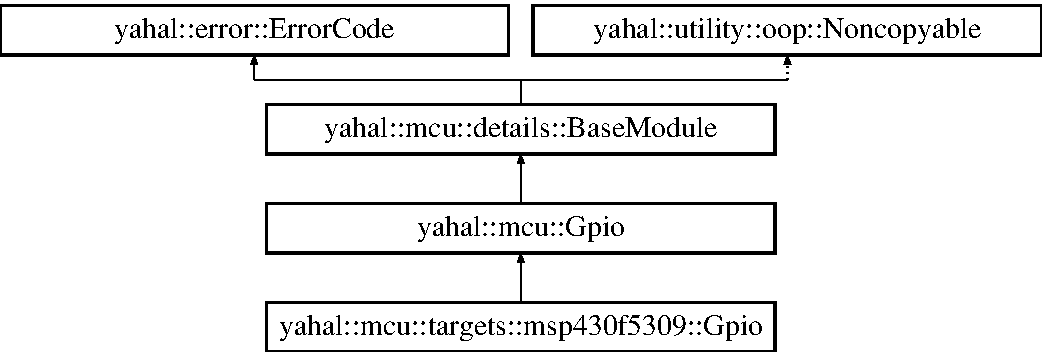
\includegraphics[height=4.000000cm]{classyahal_1_1mcu_1_1_gpio}
\end{center}
\end{figure}
\subsection*{Classes}
\begin{DoxyCompactItemize}
\item 
struct \hyperlink{structyahal_1_1mcu_1_1_gpio_1_1_direction}{Direction}
\begin{DoxyCompactList}\small\item\em \hyperlink{structyahal_1_1mcu_1_1_gpio_1_1_direction}{Direction} of G\+P\+I\+O pins. \end{DoxyCompactList}\item 
struct \hyperlink{structyahal_1_1mcu_1_1_gpio_1_1_error}{Error}
\begin{DoxyCompactList}\small\item\em G\+P\+I\+O errors. \end{DoxyCompactList}\item 
class \hyperlink{classyahal_1_1mcu_1_1_gpio_1_1_port}{Port}
\begin{DoxyCompactList}\small\item\em Base class for all G\+P\+I\+O Ports. \end{DoxyCompactList}\item 
struct \hyperlink{structyahal_1_1mcu_1_1_gpio_1_1_resistor}{Resistor}
\begin{DoxyCompactList}\small\item\em Pull-\/up and pull-\/down resistor configuration. \end{DoxyCompactList}\end{DoxyCompactItemize}
\subsection*{Public Member Functions}
\begin{DoxyCompactItemize}
\item 
\hypertarget{classyahal_1_1mcu_1_1_gpio_ae479c2a3403911b60310bf0c57594dcd}{}virtual \hyperlink{classyahal_1_1mcu_1_1_gpio_1_1_port}{Port} \& \hyperlink{classyahal_1_1mcu_1_1_gpio_ae479c2a3403911b60310bf0c57594dcd}{port} (uint8\+\_\+t port\+Number)=0\label{classyahal_1_1mcu_1_1_gpio_ae479c2a3403911b60310bf0c57594dcd}

\begin{DoxyCompactList}\small\item\em Return reference to port. \end{DoxyCompactList}\item 
\hyperlink{classyahal_1_1mcu_1_1_gpio_1_1_port}{Port} \& \hyperlink{classyahal_1_1mcu_1_1_gpio_add77eaf55d6aad1987e223edf85d4c56}{operator\mbox{[}$\,$\mbox{]}} (uint8\+\_\+t port\+Number)
\begin{DoxyCompactList}\small\item\em Inline wrapper for function \hyperlink{classyahal_1_1mcu_1_1_gpio_ae479c2a3403911b60310bf0c57594dcd}{port(uint8\+\_\+t port\+Number)}. \end{DoxyCompactList}\end{DoxyCompactItemize}
\subsection*{Additional Inherited Members}


\subsection{Detailed Description}
Base class for G\+P\+I\+O modules. 

Definition at line 47 of file gpio.\+hpp.



\subsection{Member Function Documentation}
\hypertarget{classyahal_1_1mcu_1_1_gpio_add77eaf55d6aad1987e223edf85d4c56}{}\index{yahal\+::mcu\+::\+Gpio@{yahal\+::mcu\+::\+Gpio}!operator\mbox{[}$\,$\mbox{]}@{operator[]}}
\index{operator\mbox{[}$\,$\mbox{]}@{operator[]}!yahal\+::mcu\+::\+Gpio@{yahal\+::mcu\+::\+Gpio}}
\subsubsection[{operator[](uint8\+\_\+t port\+Number)}]{\setlength{\rightskip}{0pt plus 5cm}{\bf Port}\& yahal\+::mcu\+::\+Gpio\+::operator\mbox{[}$\,$\mbox{]} (
\begin{DoxyParamCaption}
\item[{uint8\+\_\+t}]{port\+Number}
\end{DoxyParamCaption}
)\hspace{0.3cm}{\ttfamily [inline]}}\label{classyahal_1_1mcu_1_1_gpio_add77eaf55d6aad1987e223edf85d4c56}


Inline wrapper for function \hyperlink{classyahal_1_1mcu_1_1_gpio_ae479c2a3403911b60310bf0c57594dcd}{port(uint8\+\_\+t port\+Number)}. 

For less verbose code. 

Definition at line 95 of file gpio.\+hpp.



The documentation for this class was generated from the following file\+:\begin{DoxyCompactItemize}
\item 
/home/andy/\+Documentos/\+Source/yahal/mcu/modules/gpio/gpio.\+hpp\end{DoxyCompactItemize}

\hypertarget{structyahal_1_1mcu_1_1_irq_1_1_i2_c}{}\section{yahal\+:\+:mcu\+:\+:Irq\+:\+:I2\+C Struct Reference}
\label{structyahal_1_1mcu_1_1_irq_1_1_i2_c}\index{yahal\+::mcu\+::\+Irq\+::\+I2\+C@{yahal\+::mcu\+::\+Irq\+::\+I2\+C}}
\subsection*{Public Types}
\begin{DoxyCompactItemize}
\item 
\hypertarget{structyahal_1_1mcu_1_1_irq_1_1_i2_c_acd51c57af795744492ee0c003e79318a}{}enum {\bfseries type} \{ {\bfseries T\+X\+\_\+\+B\+U\+F\+F\+E\+R\+\_\+\+E\+M\+P\+T\+Y}, 
{\bfseries R\+X\+\_\+\+B\+U\+F\+F\+E\+R\+\_\+\+F\+U\+L\+L}, 
{\bfseries R\+E\+C\+E\+I\+V\+E\+D\+\_\+\+N\+A\+C\+K}, 
{\bfseries R\+E\+C\+E\+I\+V\+E\+D\+\_\+\+S\+T\+A\+R\+T}
 \}\label{structyahal_1_1mcu_1_1_irq_1_1_i2_c_acd51c57af795744492ee0c003e79318a}

\end{DoxyCompactItemize}


\subsection{Detailed Description}


Definition at line 66 of file irq.\+hpp.



The documentation for this struct was generated from the following file\+:\begin{DoxyCompactItemize}
\item 
/home/andy/\+Documentos/\+Source/yahal/mcu/modules/irq/irq.\+hpp\end{DoxyCompactItemize}

\hypertarget{classyahal_1_1mcu_1_1details_1_1_i2_c__common}{}\section{yahal\+:\+:mcu\+:\+:details\+:\+:I2\+C\+\_\+common Class Reference}
\label{classyahal_1_1mcu_1_1details_1_1_i2_c__common}\index{yahal\+::mcu\+::details\+::\+I2\+C\+\_\+common@{yahal\+::mcu\+::details\+::\+I2\+C\+\_\+common}}


Base class for all I2\+C modules.  




{\ttfamily \#include $<$i2c\+\_\+common.\+hpp$>$}

Inheritance diagram for yahal\+:\+:mcu\+:\+:details\+:\+:I2\+C\+\_\+common\+:\begin{figure}[H]
\begin{center}
\leavevmode
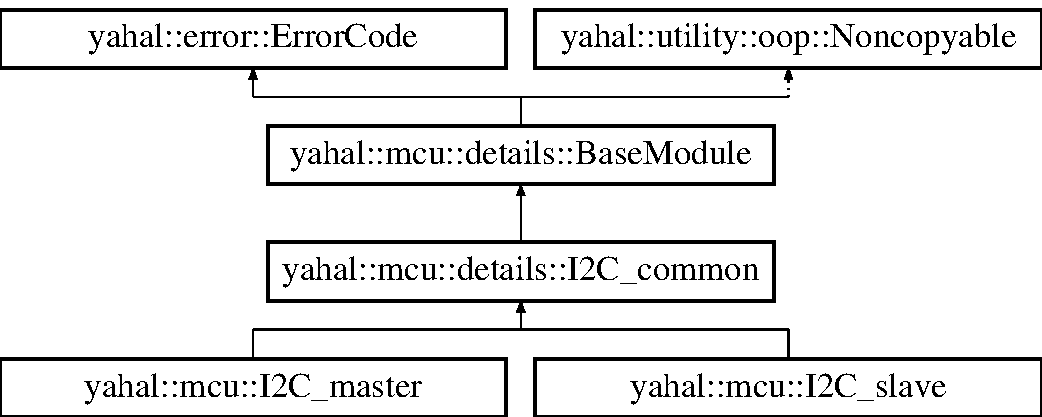
\includegraphics[height=4.000000cm]{classyahal_1_1mcu_1_1details_1_1_i2_c__common}
\end{center}
\end{figure}
\subsection*{Classes}
\begin{DoxyCompactItemize}
\item 
struct \hyperlink{structyahal_1_1mcu_1_1details_1_1_i2_c__common_1_1_direction}{Direction}
\begin{DoxyCompactList}\small\item\em I/\+O operation direction. \end{DoxyCompactList}\item 
struct \hyperlink{structyahal_1_1mcu_1_1details_1_1_i2_c__common_1_1_error}{Error}
\begin{DoxyCompactList}\small\item\em \hyperlink{structyahal_1_1mcu_1_1details_1_1_i2_c__common_1_1_error}{Error} codes for I2\+C. \end{DoxyCompactList}\end{DoxyCompactItemize}
\subsection*{Protected Member Functions}
\begin{DoxyCompactItemize}
\item 
virtual void \hyperlink{classyahal_1_1mcu_1_1details_1_1_i2_c__common_a2d57008663c00d17865d6dcdf9114253}{write\+Buffer\+T\+X} (uint8\+\_\+t byte)=0
\begin{DoxyCompactList}\small\item\em Prepare write. \end{DoxyCompactList}\item 
virtual uint8\+\_\+t \hyperlink{classyahal_1_1mcu_1_1details_1_1_i2_c__common_a98bc3518e3a4fad5a2e942853550ccb9}{read\+Buffer\+R\+X} (void)=0
\begin{DoxyCompactList}\small\item\em Finish read. \end{DoxyCompactList}\end{DoxyCompactItemize}
\subsection*{Additional Inherited Members}


\subsection{Detailed Description}
Base class for all I2\+C modules. 

This virtual class implements all common elements to all I2\+C operation modes. 

Definition at line 49 of file i2c\+\_\+common.\+hpp.



\subsection{Member Function Documentation}
\hypertarget{classyahal_1_1mcu_1_1details_1_1_i2_c__common_a98bc3518e3a4fad5a2e942853550ccb9}{}\index{yahal\+::mcu\+::details\+::\+I2\+C\+\_\+common@{yahal\+::mcu\+::details\+::\+I2\+C\+\_\+common}!read\+Buffer\+R\+X@{read\+Buffer\+R\+X}}
\index{read\+Buffer\+R\+X@{read\+Buffer\+R\+X}!yahal\+::mcu\+::details\+::\+I2\+C\+\_\+common@{yahal\+::mcu\+::details\+::\+I2\+C\+\_\+common}}
\subsubsection[{read\+Buffer\+R\+X(void)=0}]{\setlength{\rightskip}{0pt plus 5cm}virtual uint8\+\_\+t yahal\+::mcu\+::details\+::\+I2\+C\+\_\+common\+::read\+Buffer\+R\+X (
\begin{DoxyParamCaption}
\item[{void}]{}
\end{DoxyParamCaption}
)\hspace{0.3cm}{\ttfamily [protected]}, {\ttfamily [pure virtual]}}\label{classyahal_1_1mcu_1_1details_1_1_i2_c__common_a98bc3518e3a4fad5a2e942853550ccb9}


Finish read. 

\hypertarget{classyahal_1_1mcu_1_1details_1_1_i2_c__common_a2d57008663c00d17865d6dcdf9114253}{}\index{yahal\+::mcu\+::details\+::\+I2\+C\+\_\+common@{yahal\+::mcu\+::details\+::\+I2\+C\+\_\+common}!write\+Buffer\+T\+X@{write\+Buffer\+T\+X}}
\index{write\+Buffer\+T\+X@{write\+Buffer\+T\+X}!yahal\+::mcu\+::details\+::\+I2\+C\+\_\+common@{yahal\+::mcu\+::details\+::\+I2\+C\+\_\+common}}
\subsubsection[{write\+Buffer\+T\+X(uint8\+\_\+t byte)=0}]{\setlength{\rightskip}{0pt plus 5cm}virtual void yahal\+::mcu\+::details\+::\+I2\+C\+\_\+common\+::write\+Buffer\+T\+X (
\begin{DoxyParamCaption}
\item[{uint8\+\_\+t}]{byte}
\end{DoxyParamCaption}
)\hspace{0.3cm}{\ttfamily [protected]}, {\ttfamily [pure virtual]}}\label{classyahal_1_1mcu_1_1details_1_1_i2_c__common_a2d57008663c00d17865d6dcdf9114253}


Prepare write. 



The documentation for this class was generated from the following file\+:\begin{DoxyCompactItemize}
\item 
/home/andy/\+Documentos/\+Source/yahal/mcu/modules/i2c/i2c\+\_\+common.\+hpp\end{DoxyCompactItemize}

\hypertarget{classyahal_1_1mcu_1_1_i2_c__master}{}\section{yahal\+:\+:mcu\+:\+:I2\+C\+\_\+master Class Reference}
\label{classyahal_1_1mcu_1_1_i2_c__master}\index{yahal\+::mcu\+::\+I2\+C\+\_\+master@{yahal\+::mcu\+::\+I2\+C\+\_\+master}}


Base class for all I2\+C Masters.  




{\ttfamily \#include $<$i2c\+\_\+master.\+hpp$>$}

Inheritance diagram for yahal\+:\+:mcu\+:\+:I2\+C\+\_\+master\+:\begin{figure}[H]
\begin{center}
\leavevmode
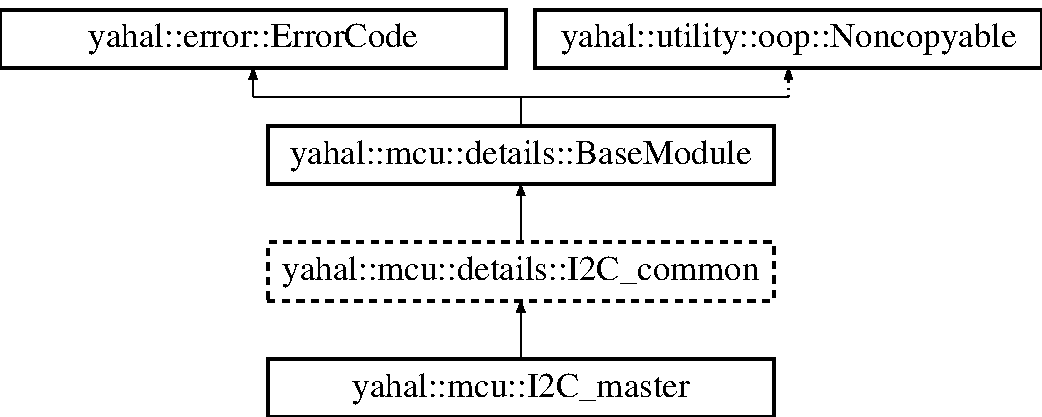
\includegraphics[height=4.000000cm]{classyahal_1_1mcu_1_1_i2_c__master}
\end{center}
\end{figure}
\subsection*{Public Member Functions}
\begin{DoxyCompactItemize}
\item 
\hypertarget{classyahal_1_1mcu_1_1_i2_c__master_a50d197cc66ef0825bed15f67b16a701b}{}virtual bool \hyperlink{classyahal_1_1mcu_1_1_i2_c__master_a50d197cc66ef0825bed15f67b16a701b}{write\+Register} (uint8\+\_\+t slave\+Address, uint8\+\_\+t register\+Address, uint8\+\_\+t $\ast$data, std\+::size\+\_\+t size)\label{classyahal_1_1mcu_1_1_i2_c__master_a50d197cc66ef0825bed15f67b16a701b}

\begin{DoxyCompactList}\small\item\em ====================================================================================== W\+R\+I\+T\+E \end{DoxyCompactList}\item 
\hypertarget{classyahal_1_1mcu_1_1_i2_c__master_a7ea7f55c54c1f6bcb7224ab06dc45d64}{}virtual bool {\bfseries write} (uint8\+\_\+t slave\+Address, uint8\+\_\+t $\ast$data, std\+::size\+\_\+t size)\label{classyahal_1_1mcu_1_1_i2_c__master_a7ea7f55c54c1f6bcb7224ab06dc45d64}

\item 
\hypertarget{classyahal_1_1mcu_1_1_i2_c__master_a63300f623b504d6ec969b4e76764fb02}{}virtual bool \hyperlink{classyahal_1_1mcu_1_1_i2_c__master_a63300f623b504d6ec969b4e76764fb02}{read\+Register} (uint8\+\_\+t slave\+Address, uint8\+\_\+t register\+Address, uint8\+\_\+t $\ast$data, std\+::size\+\_\+t size)\label{classyahal_1_1mcu_1_1_i2_c__master_a63300f623b504d6ec969b4e76764fb02}

\begin{DoxyCompactList}\small\item\em ======================================================================================= R\+E\+A\+D \end{DoxyCompactList}\item 
\hypertarget{classyahal_1_1mcu_1_1_i2_c__master_a4550ee5d6613d0fd76ea1750b3ed5935}{}virtual bool {\bfseries read} (uint8\+\_\+t slave\+Address, uint8\+\_\+t $\ast$data, std\+::size\+\_\+t size)\label{classyahal_1_1mcu_1_1_i2_c__master_a4550ee5d6613d0fd76ea1750b3ed5935}

\item 
\hypertarget{classyahal_1_1mcu_1_1_i2_c__master_a5917071910d96d6b2f941877daf09d13}{}virtual bool \hyperlink{classyahal_1_1mcu_1_1_i2_c__master_a5917071910d96d6b2f941877daf09d13}{is\+Slave\+Present} (uint8\+\_\+t slave\+Address)\label{classyahal_1_1mcu_1_1_i2_c__master_a5917071910d96d6b2f941877daf09d13}

\begin{DoxyCompactList}\small\item\em ==================================================================================== U\+T\+I\+L\+I\+T\+Y \end{DoxyCompactList}\item 
\hypertarget{classyahal_1_1mcu_1_1_i2_c__master_a96a0c05ef0cbfc1701571ee32d9901b7}{}{\footnotesize template$<$typename T $>$ }\\bool {\bfseries write\+Register} (uint8\+\_\+t slave\+Addr, uint8\+\_\+t reg\+Addr, T \&data)\label{classyahal_1_1mcu_1_1_i2_c__master_a96a0c05ef0cbfc1701571ee32d9901b7}

\item 
\hypertarget{classyahal_1_1mcu_1_1_i2_c__master_ab04427f7a2c279f85897c569980e5028}{}{\footnotesize template$<$typename T $>$ }\\bool {\bfseries write} (uint8\+\_\+t slave\+Addr, T \&data)\label{classyahal_1_1mcu_1_1_i2_c__master_ab04427f7a2c279f85897c569980e5028}

\item 
\hypertarget{classyahal_1_1mcu_1_1_i2_c__master_adfe3bfaf21ca6242b136d7a98801c2d1}{}{\footnotesize template$<$typename T $>$ }\\bool {\bfseries read\+Register} (uint8\+\_\+t slave\+Addr, uint8\+\_\+t reg\+Addr, T \&data)\label{classyahal_1_1mcu_1_1_i2_c__master_adfe3bfaf21ca6242b136d7a98801c2d1}

\item 
\hypertarget{classyahal_1_1mcu_1_1_i2_c__master_a47a3ab29396a9a55e219420b16e93294}{}{\footnotesize template$<$typename T $>$ }\\bool {\bfseries read} (uint8\+\_\+t slave\+Addr, T \&data)\label{classyahal_1_1mcu_1_1_i2_c__master_a47a3ab29396a9a55e219420b16e93294}

\item 
\hypertarget{classyahal_1_1mcu_1_1_i2_c__master_af7b36228ed09e8aac886f4d4325b1c1e}{}virtual void \hyperlink{classyahal_1_1mcu_1_1_i2_c__master_af7b36228ed09e8aac886f4d4325b1c1e}{handle\+Buffer\+T\+X\+Empty} (void)\label{classyahal_1_1mcu_1_1_i2_c__master_af7b36228ed09e8aac886f4d4325b1c1e}

\begin{DoxyCompactList}\small\item\em ======================================================================================== I\+R\+Q \end{DoxyCompactList}\item 
\hypertarget{classyahal_1_1mcu_1_1_i2_c__master_a0902de640df4a6a0a95f5ad526c20495}{}virtual void {\bfseries handle\+Buffer\+R\+X\+Full} (void)\label{classyahal_1_1mcu_1_1_i2_c__master_a0902de640df4a6a0a95f5ad526c20495}

\item 
\hypertarget{classyahal_1_1mcu_1_1_i2_c__master_a2a3d46c9ad4ef297f05ec628e86293ea}{}virtual void {\bfseries handle\+Received\+Nack} (void)\label{classyahal_1_1mcu_1_1_i2_c__master_a2a3d46c9ad4ef297f05ec628e86293ea}

\end{DoxyCompactItemize}
\subsection*{Protected Member Functions}
\begin{DoxyCompactItemize}
\item 
\hypertarget{classyahal_1_1mcu_1_1_i2_c__master_a515d0a5f65c651a5a50f0b1188e5c76c}{}virtual void \hyperlink{classyahal_1_1mcu_1_1_i2_c__master_a515d0a5f65c651a5a50f0b1188e5c76c}{start} (uint8\+\_\+t slave\+Address, Direction\+::\+Type direction)=0\label{classyahal_1_1mcu_1_1_i2_c__master_a515d0a5f65c651a5a50f0b1188e5c76c}

\begin{DoxyCompactList}\small\item\em ====================================================================== M\+O\+D\+U\+L\+E I\+M\+P\+L\+E\+M\+E\+N\+T\+A\+T\+I\+O\+N \end{DoxyCompactList}\item 
\hypertarget{classyahal_1_1mcu_1_1_i2_c__master_a6e6917ff19fb323e899970dd511a533b}{}virtual void {\bfseries stop} (void)=0\label{classyahal_1_1mcu_1_1_i2_c__master_a6e6917ff19fb323e899970dd511a533b}

\item 
\hypertarget{classyahal_1_1mcu_1_1_i2_c__master_ad8a78ad95cebfbd6e4140456a5e78bec}{}virtual void {\bfseries await\+Transmission\+End} (void)=0\label{classyahal_1_1mcu_1_1_i2_c__master_ad8a78ad95cebfbd6e4140456a5e78bec}

\end{DoxyCompactItemize}
\subsection*{Additional Inherited Members}


\subsection{Detailed Description}
Base class for all I2\+C Masters. 

Definition at line 50 of file i2c\+\_\+master.\+hpp.



The documentation for this class was generated from the following files\+:\begin{DoxyCompactItemize}
\item 
/home/andy/\+Documentos/\+Source/yahal/mcu/modules/i2c/i2c\+\_\+master.\+hpp\item 
/home/andy/\+Documentos/\+Source/yahal/mcu/hwemulation/i2c/i2c\+\_\+master.\+cpp\end{DoxyCompactItemize}

\hypertarget{classyahal_1_1mcu_1_1_i2_c__slave}{}\section{yahal\+:\+:mcu\+:\+:I2\+C\+\_\+slave Class Reference}
\label{classyahal_1_1mcu_1_1_i2_c__slave}\index{yahal\+::mcu\+::\+I2\+C\+\_\+slave@{yahal\+::mcu\+::\+I2\+C\+\_\+slave}}


Base class for all I2\+C slaves.  




{\ttfamily \#include $<$i2c\+\_\+slave.\+hpp$>$}

Inheritance diagram for yahal\+:\+:mcu\+:\+:I2\+C\+\_\+slave\+:\begin{figure}[H]
\begin{center}
\leavevmode
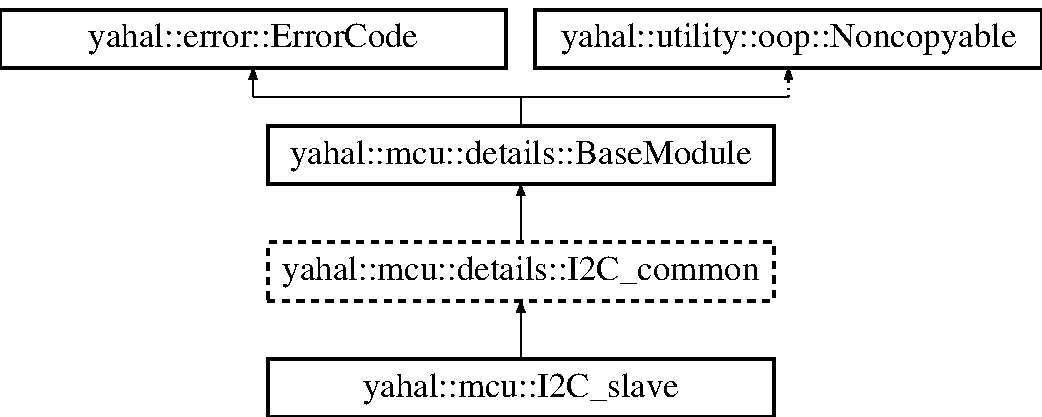
\includegraphics[height=4.000000cm]{classyahal_1_1mcu_1_1_i2_c__slave}
\end{center}
\end{figure}
\subsection*{Public Member Functions}
\begin{DoxyCompactItemize}
\item 
\hypertarget{classyahal_1_1mcu_1_1_i2_c__slave_a89a2c6293aab02189e1140082c3a0ada}{}virtual void {\bfseries handle\+Received\+Start} (void)\label{classyahal_1_1mcu_1_1_i2_c__slave_a89a2c6293aab02189e1140082c3a0ada}

\item 
\hypertarget{classyahal_1_1mcu_1_1_i2_c__slave_aff9257fb7bba6935470e7e4df7be665a}{}virtual void {\bfseries handle\+Received\+Stop} (void)\label{classyahal_1_1mcu_1_1_i2_c__slave_aff9257fb7bba6935470e7e4df7be665a}

\item 
\hypertarget{classyahal_1_1mcu_1_1_i2_c__slave_aaf745b91c3f902f135219c385e082c12}{}virtual void {\bfseries handle\+Buffer\+T\+X\+Empty} (void)\label{classyahal_1_1mcu_1_1_i2_c__slave_aaf745b91c3f902f135219c385e082c12}

\item 
\hypertarget{classyahal_1_1mcu_1_1_i2_c__slave_af2bc4067c1e2c8cc499dde9bfd55f9f2}{}virtual void {\bfseries handle\+Buffer\+R\+X\+Full} (void)\label{classyahal_1_1mcu_1_1_i2_c__slave_af2bc4067c1e2c8cc499dde9bfd55f9f2}

\item 
\hypertarget{classyahal_1_1mcu_1_1_i2_c__slave_ab21ae123a6dd0ced188cfd78b14c6de8}{}void {\bfseries set\+Callback\+Received\+Start} (void($\ast$fp\+Call\+On\+Event)(Direction\+::\+Type))\label{classyahal_1_1mcu_1_1_i2_c__slave_ab21ae123a6dd0ced188cfd78b14c6de8}

\item 
\hypertarget{classyahal_1_1mcu_1_1_i2_c__slave_a9cd6542bef603a8bc1da8ba1ba1c5f41}{}void {\bfseries set\+Callback\+Received\+Stop} (void($\ast$fp\+Call\+On\+Event)(void))\label{classyahal_1_1mcu_1_1_i2_c__slave_a9cd6542bef603a8bc1da8ba1ba1c5f41}

\item 
\hypertarget{classyahal_1_1mcu_1_1_i2_c__slave_a78a651cf27799db59250c2a5646b6502}{}void {\bfseries set\+Callback\+Byte\+Received} (void($\ast$fp\+Call\+On\+Event)(uint8\+\_\+t))\label{classyahal_1_1mcu_1_1_i2_c__slave_a78a651cf27799db59250c2a5646b6502}

\item 
\hypertarget{classyahal_1_1mcu_1_1_i2_c__slave_a7b266fcbfcc75dda6695d8a321e66ca4}{}void {\bfseries set\+Callback\+Byte\+Requested} (void($\ast$fp\+Call\+On\+Event)(uint8\+\_\+t \&))\label{classyahal_1_1mcu_1_1_i2_c__slave_a7b266fcbfcc75dda6695d8a321e66ca4}

\end{DoxyCompactItemize}
\subsection*{Protected Member Functions}
\begin{DoxyCompactItemize}
\item 
\hypertarget{classyahal_1_1mcu_1_1_i2_c__slave_a452c58e3bfd632a4465809eee83f7784}{}virtual bool {\bfseries is\+Incomming\+Write} (void)=0\label{classyahal_1_1mcu_1_1_i2_c__slave_a452c58e3bfd632a4465809eee83f7784}

\end{DoxyCompactItemize}
\subsection*{Additional Inherited Members}


\subsection{Detailed Description}
Base class for all I2\+C slaves. 

Definition at line 51 of file i2c\+\_\+slave.\+hpp.



The documentation for this class was generated from the following file\+:\begin{DoxyCompactItemize}
\item 
/home/andy/\+Documentos/\+Source/yahal/mcu/modules/i2c/i2c\+\_\+slave.\+hpp\end{DoxyCompactItemize}

\hypertarget{structhal_1_1sensors_1_1_ads1115_1_1_i_n_p_u_t}{}\section{hal\+:\+:sensors\+:\+:Ads1115\+:\+:I\+N\+P\+U\+T Struct Reference}
\label{structhal_1_1sensors_1_1_ads1115_1_1_i_n_p_u_t}\index{hal\+::sensors\+::\+Ads1115\+::\+I\+N\+P\+U\+T@{hal\+::sensors\+::\+Ads1115\+::\+I\+N\+P\+U\+T}}
\subsection*{Public Types}
\begin{DoxyCompactItemize}
\item 
\hypertarget{structhal_1_1sensors_1_1_ads1115_1_1_i_n_p_u_t_af2ec0c641f654669a38008104687fb9a}{}enum {\bfseries type} \{ \\*
{\bfseries A\+I\+N0\+\_\+\+A\+I\+N1} = 0b000, 
{\bfseries A\+I\+N0\+\_\+\+A\+I\+N3} = 0b001, 
{\bfseries A\+I\+N1\+\_\+\+A\+I\+N3} = 0b010, 
{\bfseries A\+I\+N2\+\_\+\+A\+I\+N3} = 0b011, 
\\*
{\bfseries A\+I\+N0\+\_\+\+G\+N\+D} = 0b100, 
{\bfseries A\+I\+N1\+\_\+\+G\+N\+D} = 0b101, 
{\bfseries A\+I\+N2\+\_\+\+G\+N\+D} = 0b110, 
{\bfseries A\+I\+N3\+\_\+\+G\+N\+D} = 0b111
 \}\label{structhal_1_1sensors_1_1_ads1115_1_1_i_n_p_u_t_af2ec0c641f654669a38008104687fb9a}

\end{DoxyCompactItemize}


\subsection{Detailed Description}


Definition at line 80 of file ads1115.\+hpp.



The documentation for this struct was generated from the following file\+:\begin{DoxyCompactItemize}
\item 
/home/andy/\+Documentos/\+Source/yahal/sensors/ads1115/ads1115.\+hpp\end{DoxyCompactItemize}

\hypertarget{classyahal_1_1mcu_1_1_irq}{}\section{yahal\+:\+:mcu\+:\+:Irq Class Reference}
\label{classyahal_1_1mcu_1_1_irq}\index{yahal\+::mcu\+::\+Irq@{yahal\+::mcu\+::\+Irq}}


Base class for all I\+R\+Q handlers.  




{\ttfamily \#include $<$irq.\+hpp$>$}

Inheritance diagram for yahal\+:\+:mcu\+:\+:Irq\+:\begin{figure}[H]
\begin{center}
\leavevmode
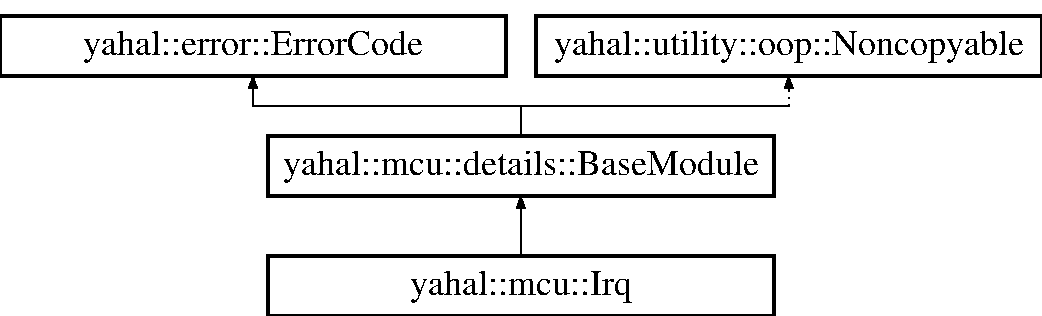
\includegraphics[height=3.000000cm]{classyahal_1_1mcu_1_1_irq}
\end{center}
\end{figure}
\subsection*{Classes}
\begin{DoxyCompactItemize}
\item 
struct \hyperlink{structyahal_1_1mcu_1_1_irq_1_1_error}{Error}
\item 
struct \hyperlink{structyahal_1_1mcu_1_1_irq_1_1_g_p_i_o}{G\+P\+I\+O}
\item 
struct \hyperlink{structyahal_1_1mcu_1_1_irq_1_1_i2_c}{I2\+C}
\item 
struct \hyperlink{structyahal_1_1mcu_1_1_irq_1_1_u_a_r_t}{U\+A\+R\+T}
\end{DoxyCompactItemize}
\subsection*{Additional Inherited Members}


\subsection{Detailed Description}
Base class for all I\+R\+Q handlers. 

Definition at line 48 of file irq.\+hpp.



The documentation for this class was generated from the following file\+:\begin{DoxyCompactItemize}
\item 
/home/andy/\+Documentos/\+Source/yahal/mcu/modules/irq/irq.\+hpp\end{DoxyCompactItemize}

\hypertarget{classhal_1_1utility_1_1_message_buffer}{}\section{hal\+:\+:utility\+:\+:Message\+Buffer$<$ T\+\_\+data, T\+\_\+buffer\+Size $>$ Class Template Reference}
\label{classhal_1_1utility_1_1_message_buffer}\index{hal\+::utility\+::\+Message\+Buffer$<$ T\+\_\+data, T\+\_\+buffer\+Size $>$@{hal\+::utility\+::\+Message\+Buffer$<$ T\+\_\+data, T\+\_\+buffer\+Size $>$}}


\subsection{Detailed Description}
\subsubsection*{template$<$class T\+\_\+data, std\+::size\+\_\+t T\+\_\+buffer\+Size$>$class hal\+::utility\+::\+Message\+Buffer$<$ T\+\_\+data, T\+\_\+buffer\+Size $>$}



Definition at line 40 of file message\+\_\+buffer.\+hpp.



The documentation for this class was generated from the following file\+:\begin{DoxyCompactItemize}
\item 
/home/andy/\+Documentos/\+Source/yahal/utility/buffer/message\+\_\+buffer.\+hpp\end{DoxyCompactItemize}

\hypertarget{classhal_1_1utility_1_1_message_stack}{}\section{hal\+:\+:utility\+:\+:Message\+Stack$<$ T\+\_\+data, T\+\_\+stack\+Size $>$ Class Template Reference}
\label{classhal_1_1utility_1_1_message_stack}\index{hal\+::utility\+::\+Message\+Stack$<$ T\+\_\+data, T\+\_\+stack\+Size $>$@{hal\+::utility\+::\+Message\+Stack$<$ T\+\_\+data, T\+\_\+stack\+Size $>$}}


{\ttfamily \#include $<$messagestack.\+hpp$>$}



\subsection{Detailed Description}
\subsubsection*{template$<$class T\+\_\+data, std\+::size\+\_\+t T\+\_\+stack\+Size$>$class hal\+::utility\+::\+Message\+Stack$<$ T\+\_\+data, T\+\_\+stack\+Size $>$}



Definition at line 41 of file messagestack.\+hpp.



The documentation for this class was generated from the following file\+:\begin{DoxyCompactItemize}
\item 
/home/andy/\+Documentos/\+Source/yahal/mcu/utility/\hyperlink{messagestack_8hpp}{messagestack.\+hpp}\end{DoxyCompactItemize}

\hypertarget{classyahal_1_1rtos_1_1api_1_1_mutex}{}\section{yahal\+:\+:rtos\+:\+:api\+:\+:Mutex Class Reference}
\label{classyahal_1_1rtos_1_1api_1_1_mutex}\index{yahal\+::rtos\+::api\+::\+Mutex@{yahal\+::rtos\+::api\+::\+Mutex}}


Base class for all M\+U\+T\+E\+X.  




{\ttfamily \#include $<$api\+\_\+mutex.\+hpp$>$}

Inheritance diagram for yahal\+:\+:rtos\+:\+:api\+:\+:Mutex\+:\begin{figure}[H]
\begin{center}
\leavevmode
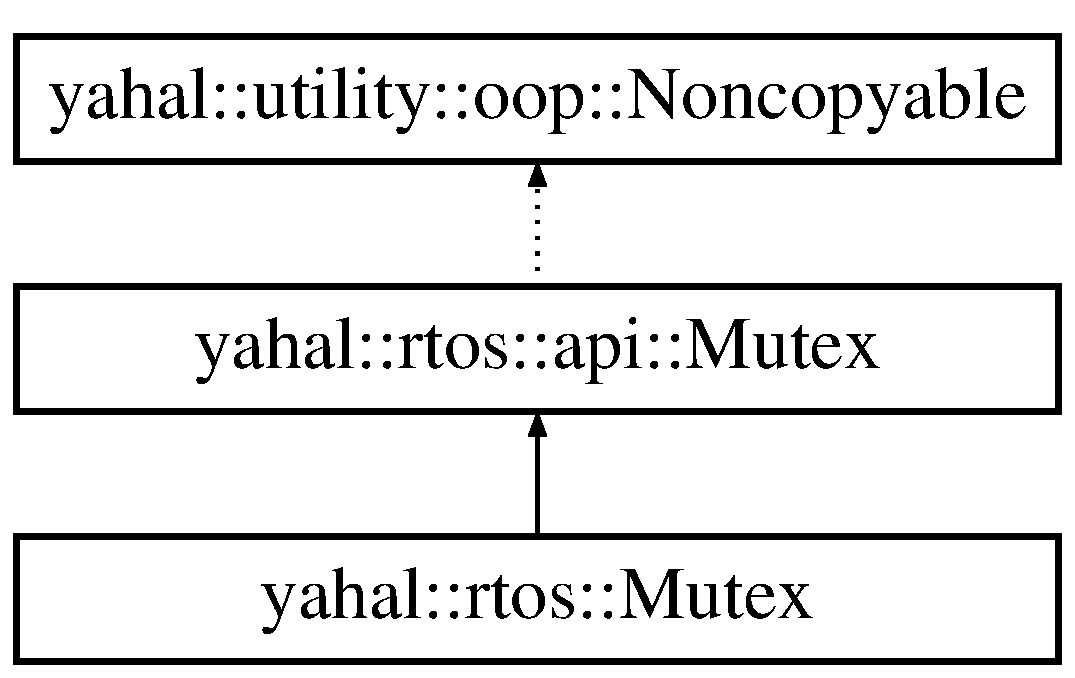
\includegraphics[height=3.000000cm]{classyahal_1_1rtos_1_1api_1_1_mutex}
\end{center}
\end{figure}
\subsection*{Public Member Functions}
\begin{DoxyCompactItemize}
\item 
\hypertarget{classyahal_1_1rtos_1_1api_1_1_mutex_a34dcfba67a052a8f4a28a513108a2920}{}virtual void {\bfseries lock} (void)=0\label{classyahal_1_1rtos_1_1api_1_1_mutex_a34dcfba67a052a8f4a28a513108a2920}

\item 
\hypertarget{classyahal_1_1rtos_1_1api_1_1_mutex_a32b7f850efd201d11dde4a98a298af68}{}virtual bool {\bfseries try\+\_\+lock} (void)=0\label{classyahal_1_1rtos_1_1api_1_1_mutex_a32b7f850efd201d11dde4a98a298af68}

\item 
\hypertarget{classyahal_1_1rtos_1_1api_1_1_mutex_ac5b67f3c507906dd24a3db27868b3b4a}{}virtual void {\bfseries unlock} (void)=0\label{classyahal_1_1rtos_1_1api_1_1_mutex_ac5b67f3c507906dd24a3db27868b3b4a}

\end{DoxyCompactItemize}


\subsection{Detailed Description}
Base class for all M\+U\+T\+E\+X. 

Definition at line 42 of file api\+\_\+mutex.\+hpp.



The documentation for this class was generated from the following file\+:\begin{DoxyCompactItemize}
\item 
/home/andy/\+Documentos/\+Source/yahal/rtos/api/api\+\_\+mutex.\+hpp\end{DoxyCompactItemize}

\hypertarget{classyahal_1_1rtos_1_1_mutex}{}\section{yahal\+:\+:rtos\+:\+:Mutex Class Reference}
\label{classyahal_1_1rtos_1_1_mutex}\index{yahal\+::rtos\+::\+Mutex@{yahal\+::rtos\+::\+Mutex}}


Does absolutely nothing.  




{\ttfamily \#include $<$empty\+\_\+mutex.\+hpp$>$}

Inheritance diagram for yahal\+:\+:rtos\+:\+:Mutex\+:\begin{figure}[H]
\begin{center}
\leavevmode
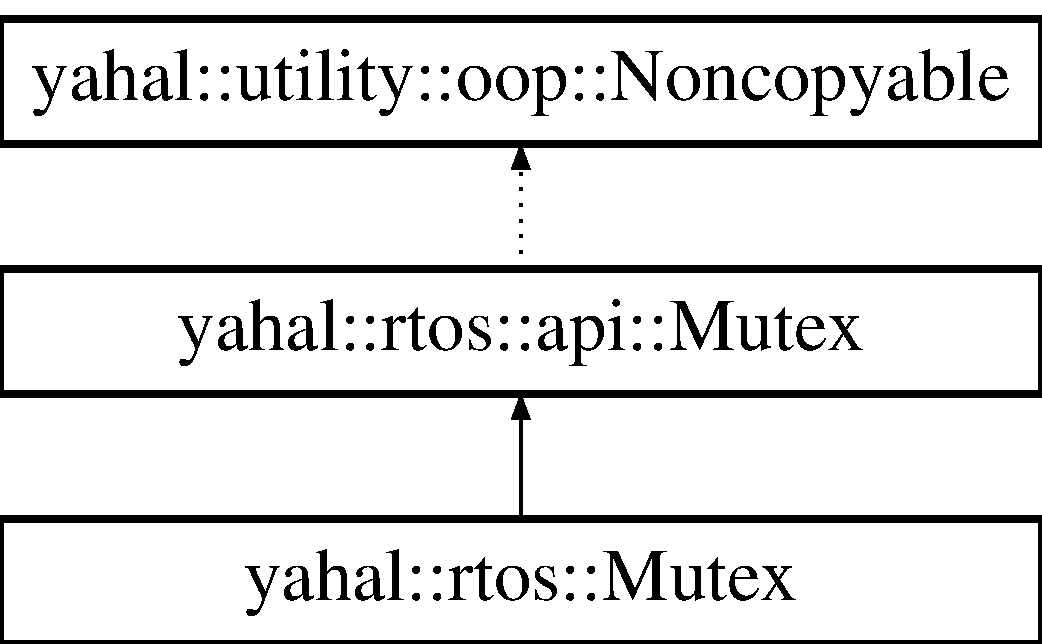
\includegraphics[height=3.000000cm]{classyahal_1_1rtos_1_1_mutex}
\end{center}
\end{figure}
\subsection*{Public Member Functions}
\begin{DoxyCompactItemize}
\item 
\hypertarget{classyahal_1_1rtos_1_1_mutex_a43df7d0b3e52ab1dc78474bc63dbe67f}{}void {\bfseries lock} (void)\label{classyahal_1_1rtos_1_1_mutex_a43df7d0b3e52ab1dc78474bc63dbe67f}

\item 
\hypertarget{classyahal_1_1rtos_1_1_mutex_a7f5d68e7c4941f8be08a11b3d6ecf0e8}{}bool {\bfseries try\+\_\+lock} (void)\label{classyahal_1_1rtos_1_1_mutex_a7f5d68e7c4941f8be08a11b3d6ecf0e8}

\item 
\hypertarget{classyahal_1_1rtos_1_1_mutex_a34569c57fc1d2366560f588d6e451a46}{}void {\bfseries unlock} (void)\label{classyahal_1_1rtos_1_1_mutex_a34569c57fc1d2366560f588d6e451a46}

\end{DoxyCompactItemize}


\subsection{Detailed Description}
Does absolutely nothing. 

Definition at line 47 of file empty\+\_\+mutex.\+hpp.



The documentation for this class was generated from the following file\+:\begin{DoxyCompactItemize}
\item 
/home/andy/\+Documentos/\+Source/yahal/rtos/implementations/empty/empty\+\_\+mutex.\+hpp\end{DoxyCompactItemize}

\hypertarget{classyahal_1_1utility_1_1oop_1_1_noncopyable}{}\section{yahal\+:\+:utility\+:\+:oop\+:\+:Noncopyable Class Reference}
\label{classyahal_1_1utility_1_1oop_1_1_noncopyable}\index{yahal\+::utility\+::oop\+::\+Noncopyable@{yahal\+::utility\+::oop\+::\+Noncopyable}}


Non copyable base class.  




{\ttfamily \#include $<$noncopyable.\+hpp$>$}

Inheritance diagram for yahal\+:\+:utility\+:\+:oop\+:\+:Noncopyable\+:\begin{figure}[H]
\begin{center}
\leavevmode
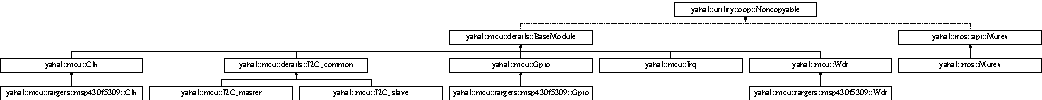
\includegraphics[height=1.350211cm]{classyahal_1_1utility_1_1oop_1_1_noncopyable}
\end{center}
\end{figure}


\subsection{Detailed Description}
Non copyable base class. 

Each class that inherits from this class can not be copied. Its constructor and asignment operator are protected and private respectively. $\ast$ 

Definition at line 44 of file noncopyable.\+hpp.



The documentation for this class was generated from the following file\+:\begin{DoxyCompactItemize}
\item 
/home/andy/\+Documentos/\+Source/yahal/utility/oop/noncopyable.\+hpp\end{DoxyCompactItemize}

\hypertarget{classyahal_1_1mcu_1_1_gpio_1_1_port_1_1_pin}{}\section{yahal\+:\+:mcu\+:\+:Gpio\+:\+:Port\+:\+:Pin Class Reference}
\label{classyahal_1_1mcu_1_1_gpio_1_1_port_1_1_pin}\index{yahal\+::mcu\+::\+Gpio\+::\+Port\+::\+Pin@{yahal\+::mcu\+::\+Gpio\+::\+Port\+::\+Pin}}


Base class for all G\+P\+I\+O Pins.  




{\ttfamily \#include $<$gpio.\+hpp$>$}

\subsection*{Public Member Functions}
\begin{DoxyCompactItemize}
\item 
\hypertarget{classyahal_1_1mcu_1_1_gpio_1_1_port_1_1_pin_a7222a8a899df5f52afb9f051ff37600f}{}{\bfseries Pin} (\hyperlink{classyahal_1_1mcu_1_1_gpio_1_1_port}{yahal\+::mcu\+::\+Gpio\+::\+Port} \&\hyperlink{classyahal_1_1mcu_1_1_gpio_ae479c2a3403911b60310bf0c57594dcd}{port}, uint8\+\_\+t pin\+Number)\label{classyahal_1_1mcu_1_1_gpio_1_1_port_1_1_pin_a7222a8a899df5f52afb9f051ff37600f}

\item 
\hypertarget{classyahal_1_1mcu_1_1_gpio_1_1_port_1_1_pin_aa14906a4f396defe53795836c79bb522}{}bool {\bfseries config} (Direction\+::\+Type direction=Direction\+::\+I\+N\+P\+U\+T, Resistor\+::\+Type resistor=Resistor\+::\+D\+I\+S\+A\+B\+L\+E\+D)\label{classyahal_1_1mcu_1_1_gpio_1_1_port_1_1_pin_aa14906a4f396defe53795836c79bb522}

\item 
\hypertarget{classyahal_1_1mcu_1_1_gpio_1_1_port_1_1_pin_aa85e73ccf2321a3677f726d9cd26ba6e}{}void {\bfseries set} (bool b)\label{classyahal_1_1mcu_1_1_gpio_1_1_port_1_1_pin_aa85e73ccf2321a3677f726d9cd26ba6e}

\item 
\hypertarget{classyahal_1_1mcu_1_1_gpio_1_1_port_1_1_pin_a2e61bdd78fb21e0fafd57467547d2492}{}bool {\bfseries get} () const \label{classyahal_1_1mcu_1_1_gpio_1_1_port_1_1_pin_a2e61bdd78fb21e0fafd57467547d2492}

\item 
\hypertarget{classyahal_1_1mcu_1_1_gpio_1_1_port_1_1_pin_a217d8e25f291766274f42706583d4cd1}{}bool {\bfseries get\+Output} () const \label{classyahal_1_1mcu_1_1_gpio_1_1_port_1_1_pin_a217d8e25f291766274f42706583d4cd1}

\item 
\hypertarget{classyahal_1_1mcu_1_1_gpio_1_1_port_1_1_pin_a56aec5c48c03afb52211da1d55a5f400}{}void {\bfseries toggle} (void)\label{classyahal_1_1mcu_1_1_gpio_1_1_port_1_1_pin_a56aec5c48c03afb52211da1d55a5f400}

\end{DoxyCompactItemize}


\subsection{Detailed Description}
Base class for all G\+P\+I\+O Pins. 

Declared inside \hyperlink{classyahal_1_1mcu_1_1_gpio_1_1_port}{Gpio\+::\+Port} 

Definition at line 136 of file gpio.\+hpp.



The documentation for this class was generated from the following files\+:\begin{DoxyCompactItemize}
\item 
/home/andy/\+Documentos/\+Source/yahal/mcu/modules/gpio/gpio.\+hpp\item 
/home/andy/\+Documentos/\+Source/yahal/mcu/modules/gpio/gpio.\+cpp\end{DoxyCompactItemize}

\hypertarget{classyahal_1_1mcu_1_1_gpio_1_1_port}{}\section{yahal\+:\+:mcu\+:\+:Gpio\+:\+:Port Class Reference}
\label{classyahal_1_1mcu_1_1_gpio_1_1_port}\index{yahal\+::mcu\+::\+Gpio\+::\+Port@{yahal\+::mcu\+::\+Gpio\+::\+Port}}


Base class for all G\+P\+I\+O Ports.  




{\ttfamily \#include $<$gpio.\+hpp$>$}

\subsection*{Classes}
\begin{DoxyCompactItemize}
\item 
class \hyperlink{classyahal_1_1mcu_1_1_gpio_1_1_port_1_1_pin}{Pin}
\begin{DoxyCompactList}\small\item\em Base class for all G\+P\+I\+O Pins. \end{DoxyCompactList}\end{DoxyCompactItemize}
\subsection*{Public Member Functions}
\begin{DoxyCompactItemize}
\item 
\hypertarget{classyahal_1_1mcu_1_1_gpio_1_1_port_a20da8a9eded1eac1ad3163fa218e51ff}{}virtual bool {\bfseries config} (Direction\+::\+Type direction=Direction\+::\+I\+N\+P\+U\+T, Resistor\+::\+Type resistor=Resistor\+::\+D\+I\+S\+A\+B\+L\+E\+D, uint8\+\_\+t mask=0x\+F\+F)=0\label{classyahal_1_1mcu_1_1_gpio_1_1_port_a20da8a9eded1eac1ad3163fa218e51ff}

\item 
\hypertarget{classyahal_1_1mcu_1_1_gpio_1_1_port_aed59cdf9217ca14979c8473684de2fb4}{}virtual void {\bfseries set} (uint8\+\_\+t value, uint8\+\_\+t mask=0x\+F\+F)=0\label{classyahal_1_1mcu_1_1_gpio_1_1_port_aed59cdf9217ca14979c8473684de2fb4}

\item 
\hypertarget{classyahal_1_1mcu_1_1_gpio_1_1_port_a22013884f0e35c548e6dcce6842c5060}{}virtual uint8\+\_\+t {\bfseries get} (uint8\+\_\+t mask=0x\+F\+F) const =0\label{classyahal_1_1mcu_1_1_gpio_1_1_port_a22013884f0e35c548e6dcce6842c5060}

\item 
\hypertarget{classyahal_1_1mcu_1_1_gpio_1_1_port_ad9b061969be01dc7d5087bbdfc938961}{}virtual uint8\+\_\+t {\bfseries get\+Output} (uint8\+\_\+t mask=0x\+F\+F) const =0\label{classyahal_1_1mcu_1_1_gpio_1_1_port_ad9b061969be01dc7d5087bbdfc938961}

\item 
\hypertarget{classyahal_1_1mcu_1_1_gpio_1_1_port_a04667de64bf79fbc59a1a7fb7051d88f}{}virtual void {\bfseries toggle} (uint8\+\_\+t mask=0x\+F\+F)\label{classyahal_1_1mcu_1_1_gpio_1_1_port_a04667de64bf79fbc59a1a7fb7051d88f}

\item 
\hyperlink{classyahal_1_1mcu_1_1_gpio_1_1_port_1_1_pin}{Pin} \hyperlink{classyahal_1_1mcu_1_1_gpio_1_1_port_aa16ce5a6eac5b549121b6036286945fe}{pin} (uint8\+\_\+t pin\+Number)
\item 
\hypertarget{classyahal_1_1mcu_1_1_gpio_1_1_port_aa3e1b5349a9c91e83ccea36e198e9fa8}{}\hyperlink{classyahal_1_1mcu_1_1_gpio_1_1_port_1_1_pin}{Pin} {\bfseries operator\mbox{[}$\,$\mbox{]}} (uint8\+\_\+t pin\+Number)\label{classyahal_1_1mcu_1_1_gpio_1_1_port_aa3e1b5349a9c91e83ccea36e198e9fa8}

\end{DoxyCompactItemize}


\subsection{Detailed Description}
Base class for all G\+P\+I\+O Ports. 

Declared inside \hyperlink{classyahal_1_1mcu_1_1_gpio}{Gpio}. 

Definition at line 104 of file gpio.\+hpp.



\subsection{Member Function Documentation}
\hypertarget{classyahal_1_1mcu_1_1_gpio_1_1_port_aa16ce5a6eac5b549121b6036286945fe}{}\index{yahal\+::mcu\+::\+Gpio\+::\+Port@{yahal\+::mcu\+::\+Gpio\+::\+Port}!pin@{pin}}
\index{pin@{pin}!yahal\+::mcu\+::\+Gpio\+::\+Port@{yahal\+::mcu\+::\+Gpio\+::\+Port}}
\subsubsection[{pin(uint8\+\_\+t pin\+Number)}]{\setlength{\rightskip}{0pt plus 5cm}{\bf yahal\+::mcu\+::\+Gpio\+::\+Port\+::\+Pin} yahal\+::mcu\+::\+Gpio\+::\+Port\+::pin (
\begin{DoxyParamCaption}
\item[{uint8\+\_\+t}]{pin\+Number}
\end{DoxyParamCaption}
)}\label{classyahal_1_1mcu_1_1_gpio_1_1_port_aa16ce5a6eac5b549121b6036286945fe}
$<$ \begin{DoxyWarning}{Warning}

\end{DoxyWarning}


Definition at line 42 of file gpio.\+cpp.



The documentation for this class was generated from the following files\+:\begin{DoxyCompactItemize}
\item 
/home/andy/\+Documentos/\+Source/yahal/mcu/modules/gpio/gpio.\+hpp\item 
/home/andy/\+Documentos/\+Source/yahal/mcu/modules/gpio/gpio.\+cpp\end{DoxyCompactItemize}

\hypertarget{structyahal_1_1mcu_1_1_gpio_1_1_resistor}{}\section{yahal\+:\+:mcu\+:\+:Gpio\+:\+:Resistor Struct Reference}
\label{structyahal_1_1mcu_1_1_gpio_1_1_resistor}\index{yahal\+::mcu\+::\+Gpio\+::\+Resistor@{yahal\+::mcu\+::\+Gpio\+::\+Resistor}}


Pull-\/up and pull-\/down resistor configuration.  




{\ttfamily \#include $<$gpio.\+hpp$>$}

\subsection*{Public Types}
\begin{DoxyCompactItemize}
\item 
\hypertarget{structyahal_1_1mcu_1_1_gpio_1_1_resistor_a8f38e7b4a5f4a55cbc6b4d6f94c0f4e5}{}enum {\bfseries Type} \{ {\bfseries D\+I\+S\+A\+B\+L\+E\+D}, 
{\bfseries P\+U\+L\+L\+U\+P}, 
{\bfseries P\+U\+L\+L\+D\+O\+W\+N}
 \}\label{structyahal_1_1mcu_1_1_gpio_1_1_resistor_a8f38e7b4a5f4a55cbc6b4d6f94c0f4e5}

\end{DoxyCompactItemize}


\subsection{Detailed Description}
Pull-\/up and pull-\/down resistor configuration. 

Definition at line 63 of file gpio.\+hpp.



The documentation for this struct was generated from the following file\+:\begin{DoxyCompactItemize}
\item 
/home/andy/\+Documentos/\+Source/yahal/mcu/modules/gpio/gpio.\+hpp\end{DoxyCompactItemize}

\hypertarget{structhal_1_1sensors_1_1_ads1115_1_1_s_c_a_l_e}{}\section{hal\+:\+:sensors\+:\+:Ads1115\+:\+:S\+C\+A\+L\+E Struct Reference}
\label{structhal_1_1sensors_1_1_ads1115_1_1_s_c_a_l_e}\index{hal\+::sensors\+::\+Ads1115\+::\+S\+C\+A\+L\+E@{hal\+::sensors\+::\+Ads1115\+::\+S\+C\+A\+L\+E}}
\subsection*{Public Types}
\begin{DoxyCompactItemize}
\item 
\hypertarget{structhal_1_1sensors_1_1_ads1115_1_1_s_c_a_l_e_a2f7392ca88e69800a9b196d46da27239}{}enum {\bfseries type} \{ \\*
{\bfseries F\+S\+\_\+6144\+\_\+\+M\+V} = 0b000, 
{\bfseries F\+S\+\_\+4096\+\_\+\+M\+V} = 0b001, 
{\bfseries F\+S\+\_\+2048\+\_\+\+M\+V} = 0b010, 
{\bfseries F\+S\+\_\+1024\+\_\+\+M\+V} = 0b011, 
\\*
{\bfseries F\+S\+\_\+512\+\_\+\+M\+V} = 0b100, 
{\bfseries F\+S\+\_\+256\+\_\+\+M\+V} = 0b111
 \}\label{structhal_1_1sensors_1_1_ads1115_1_1_s_c_a_l_e_a2f7392ca88e69800a9b196d46da27239}

\end{DoxyCompactItemize}


\subsection{Detailed Description}


Definition at line 71 of file ads1115.\+hpp.



The documentation for this struct was generated from the following file\+:\begin{DoxyCompactItemize}
\item 
/home/andy/\+Documentos/\+Source/yahal/sensors/ads1115/ads1115.\+hpp\end{DoxyCompactItemize}

\hypertarget{classhal_1_1utility_1_1_sliding_window}{}\section{hal\+:\+:utility\+:\+:Sliding\+Window$<$ T\+\_\+data, T\+\_\+buffer\+Size $>$ Class Template Reference}
\label{classhal_1_1utility_1_1_sliding_window}\index{hal\+::utility\+::\+Sliding\+Window$<$ T\+\_\+data, T\+\_\+buffer\+Size $>$@{hal\+::utility\+::\+Sliding\+Window$<$ T\+\_\+data, T\+\_\+buffer\+Size $>$}}


{\ttfamily \#include $<$sliding\+\_\+window.\+hpp$>$}



\subsection{Detailed Description}
\subsubsection*{template$<$class T\+\_\+data, std\+::size\+\_\+t T\+\_\+buffer\+Size$>$class hal\+::utility\+::\+Sliding\+Window$<$ T\+\_\+data, T\+\_\+buffer\+Size $>$}



Definition at line 39 of file sliding\+\_\+window.\+hpp.



The documentation for this class was generated from the following file\+:\begin{DoxyCompactItemize}
\item 
/home/andy/\+Documentos/\+Source/yahal/mcu/utility/\hyperlink{sliding__window_8hpp}{sliding\+\_\+window.\+hpp}\end{DoxyCompactItemize}

\hypertarget{structyahal_1_1mcu_1_1_irq_1_1_u_a_r_t}{}\section{yahal\+:\+:mcu\+:\+:Irq\+:\+:U\+A\+R\+T Struct Reference}
\label{structyahal_1_1mcu_1_1_irq_1_1_u_a_r_t}\index{yahal\+::mcu\+::\+Irq\+::\+U\+A\+R\+T@{yahal\+::mcu\+::\+Irq\+::\+U\+A\+R\+T}}
\subsection*{Public Types}
\begin{DoxyCompactItemize}
\item 
\hypertarget{structyahal_1_1mcu_1_1_irq_1_1_u_a_r_t_abaaf771ad4cd5f21a9177b95455dbc40}{}enum {\bfseries type} \{ {\bfseries R\+X}, 
{\bfseries T\+X}
 \}\label{structyahal_1_1mcu_1_1_irq_1_1_u_a_r_t_abaaf771ad4cd5f21a9177b95455dbc40}

\end{DoxyCompactItemize}


\subsection{Detailed Description}


Definition at line 74 of file irq.\+hpp.



The documentation for this struct was generated from the following file\+:\begin{DoxyCompactItemize}
\item 
/home/andy/\+Documentos/\+Source/yahal/mcu/modules/irq/irq.\+hpp\end{DoxyCompactItemize}

\hypertarget{classyahal_1_1mcu_1_1targets_1_1msp430f5309_1_1_wdt}{}\section{yahal\+:\+:mcu\+:\+:targets\+:\+:msp430f5309\+:\+:Wdt Class Reference}
\label{classyahal_1_1mcu_1_1targets_1_1msp430f5309_1_1_wdt}\index{yahal\+::mcu\+::targets\+::msp430f5309\+::\+Wdt@{yahal\+::mcu\+::targets\+::msp430f5309\+::\+Wdt}}


\begin{DoxyVerb}\end{DoxyVerb}
  




{\ttfamily \#include $<$wdt.\+hpp$>$}

Inheritance diagram for yahal\+:\+:mcu\+:\+:targets\+:\+:msp430f5309\+:\+:Wdt\+:\begin{figure}[H]
\begin{center}
\leavevmode
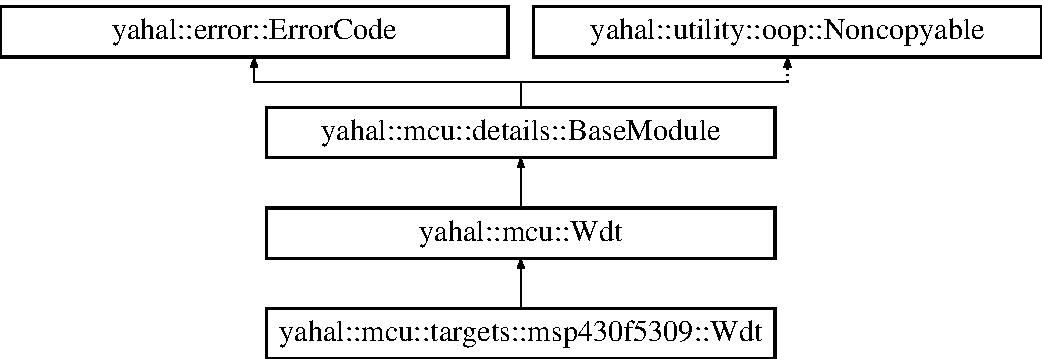
\includegraphics[height=4.000000cm]{classyahal_1_1mcu_1_1targets_1_1msp430f5309_1_1_wdt}
\end{center}
\end{figure}
\subsection*{Public Member Functions}
\begin{DoxyCompactItemize}
\item 
\hypertarget{classyahal_1_1mcu_1_1targets_1_1msp430f5309_1_1_wdt_a80cb956c417c5a477bfe07ccf7bb4356}{}void \hyperlink{classyahal_1_1mcu_1_1targets_1_1msp430f5309_1_1_wdt_a80cb956c417c5a477bfe07ccf7bb4356}{reset} (void)\label{classyahal_1_1mcu_1_1targets_1_1msp430f5309_1_1_wdt_a80cb956c417c5a477bfe07ccf7bb4356}

\begin{DoxyCompactList}\small\item\em Reset W\+D\+T counter if W\+D\+T enabled. \end{DoxyCompactList}\end{DoxyCompactItemize}
\subsection*{Additional Inherited Members}


\subsection{Detailed Description}
\begin{DoxyVerb}\end{DoxyVerb}
 

Definition at line 51 of file wdt.\+hpp.



The documentation for this class was generated from the following files\+:\begin{DoxyCompactItemize}
\item 
/home/andy/\+Documentos/\+Source/yahal/mcu/targets/msp430f5309/wdt/wdt.\+hpp\item 
/home/andy/\+Documentos/\+Source/yahal/mcu/targets/msp430f5309/wdt/wdt.\+cpp\end{DoxyCompactItemize}

\hypertarget{classyahal_1_1mcu_1_1_wdt}{}\section{yahal\+:\+:mcu\+:\+:Wdt Class Reference}
\label{classyahal_1_1mcu_1_1_wdt}\index{yahal\+::mcu\+::\+Wdt@{yahal\+::mcu\+::\+Wdt}}


Base class for all Watch Dog Timers.  




{\ttfamily \#include $<$wdt.\+hpp$>$}

Inheritance diagram for yahal\+:\+:mcu\+:\+:Wdt\+:\begin{figure}[H]
\begin{center}
\leavevmode
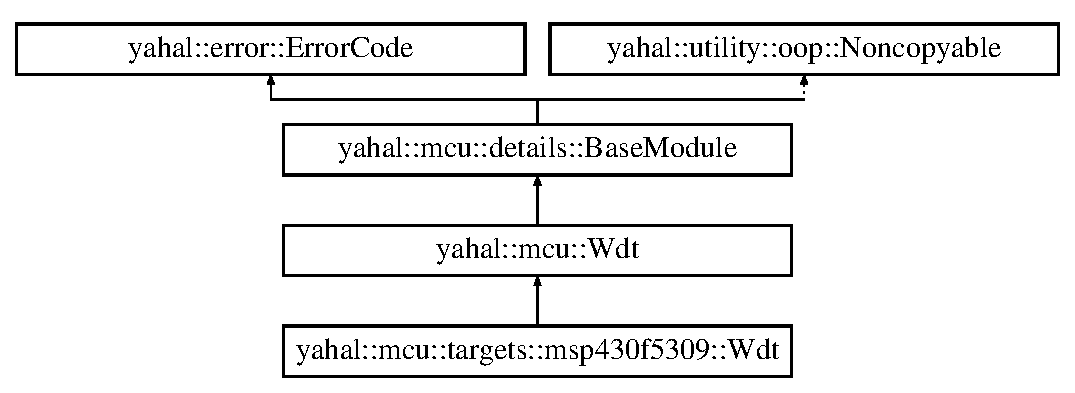
\includegraphics[height=4.000000cm]{classyahal_1_1mcu_1_1_wdt}
\end{center}
\end{figure}
\subsection*{Classes}
\begin{DoxyCompactItemize}
\item 
struct \hyperlink{structyahal_1_1mcu_1_1_wdt_1_1_error}{Error}
\end{DoxyCompactItemize}
\subsection*{Public Member Functions}
\begin{DoxyCompactItemize}
\item 
\hypertarget{classyahal_1_1mcu_1_1_wdt_a147a40273f928037437c8fefa58ed388}{}virtual void \hyperlink{classyahal_1_1mcu_1_1_wdt_a147a40273f928037437c8fefa58ed388}{reset} (void)=0\label{classyahal_1_1mcu_1_1_wdt_a147a40273f928037437c8fefa58ed388}

\begin{DoxyCompactList}\small\item\em Reset watch dog timer count. \end{DoxyCompactList}\end{DoxyCompactItemize}
\subsection*{Additional Inherited Members}


\subsection{Detailed Description}
Base class for all Watch Dog Timers. 

Definition at line 49 of file wdt.\+hpp.



The documentation for this class was generated from the following file\+:\begin{DoxyCompactItemize}
\item 
/home/andy/\+Documentos/\+Source/yahal/mcu/modules/wdt/wdt.\+hpp\end{DoxyCompactItemize}

\chapter{File Documentation}
\hypertarget{longjmp__exception_8hpp}{}\section{/home/andy/\+Documentos/\+Source/yahal/mcu/error/longjmp\+\_\+exception.hpp File Reference}
\label{longjmp__exception_8hpp}\index{/home/andy/\+Documentos/\+Source/yahal/mcu/error/longjmp\+\_\+exception.\+hpp@{/home/andy/\+Documentos/\+Source/yahal/mcu/error/longjmp\+\_\+exception.\+hpp}}
{\ttfamily \#include $<$setjmp.\+h$>$}\\*
{\ttfamily \#include $<$stdint.\+h$>$}\\*
\subsection*{Macros}
\begin{DoxyCompactItemize}
\item 
\#define \hyperlink{longjmp__exception_8hpp_ad2746371528bdf15c3910b7bf217dac0}{T\+R\+Y}
\begin{DoxyCompactList}\small\item\em \begin{DoxyVerb}ID: LONGJMP_EXCEPTION
\end{DoxyVerb}
 E\+D\+I\+T\+E\+D\+: 21-\/04-\/2015 A\+U\+T\+H\+O\+R\+: Andres Gongora \end{DoxyCompactList}\item 
\#define \hyperlink{longjmp__exception_8hpp_ae30f5c713cfa6a69c6b26492c992052b}{C\+A\+T\+C\+H}~\} else \{
\item 
\#define \hyperlink{longjmp__exception_8hpp_a4071a24a0245b51c00c9bfcf103f9c0f}{E\+N\+D\+T\+R\+Y}
\item 
\#define \hyperlink{longjmp__exception_8hpp_a32b511cadb5acde1de32c0fbf8f583c4}{T\+H\+R\+O\+W}(val)~do\{longjmp(ex\+\_\+buf\+\_\+\+\_\+, val);\}while(0)
\item 
\#define \hyperlink{longjmp__exception_8hpp_a70195a6405d6a11e6aff66ca1b6c53d7}{T\+E\+S\+T}(testvalue)~do\{if(testvalue == false) \hyperlink{longjmp__exception_8hpp_a32b511cadb5acde1de32c0fbf8f583c4}{T\+H\+R\+O\+W}(-\/1);\}while(0);
\end{DoxyCompactItemize}


\subsection{Macro Definition Documentation}
\hypertarget{longjmp__exception_8hpp_ae30f5c713cfa6a69c6b26492c992052b}{}\index{longjmp\+\_\+exception.\+hpp@{longjmp\+\_\+exception.\+hpp}!C\+A\+T\+C\+H@{C\+A\+T\+C\+H}}
\index{C\+A\+T\+C\+H@{C\+A\+T\+C\+H}!longjmp\+\_\+exception.\+hpp@{longjmp\+\_\+exception.\+hpp}}
\subsubsection[{C\+A\+T\+C\+H}]{\setlength{\rightskip}{0pt plus 5cm}\#define C\+A\+T\+C\+H~\} else \{}\label{longjmp__exception_8hpp_ae30f5c713cfa6a69c6b26492c992052b}


Definition at line 104 of file longjmp\+\_\+exception.\+hpp.

\hypertarget{longjmp__exception_8hpp_a4071a24a0245b51c00c9bfcf103f9c0f}{}\index{longjmp\+\_\+exception.\+hpp@{longjmp\+\_\+exception.\+hpp}!E\+N\+D\+T\+R\+Y@{E\+N\+D\+T\+R\+Y}}
\index{E\+N\+D\+T\+R\+Y@{E\+N\+D\+T\+R\+Y}!longjmp\+\_\+exception.\+hpp@{longjmp\+\_\+exception.\+hpp}}
\subsubsection[{E\+N\+D\+T\+R\+Y}]{\setlength{\rightskip}{0pt plus 5cm}\#define E\+N\+D\+T\+R\+Y}\label{longjmp__exception_8hpp_a4071a24a0245b51c00c9bfcf103f9c0f}
{\bfseries Value\+:}
\begin{DoxyCode}
\}                                                       \(\backslash\)
                                \}\textcolor{keywordflow}{while}(0);
\end{DoxyCode}


Definition at line 105 of file longjmp\+\_\+exception.\+hpp.

\hypertarget{longjmp__exception_8hpp_a70195a6405d6a11e6aff66ca1b6c53d7}{}\index{longjmp\+\_\+exception.\+hpp@{longjmp\+\_\+exception.\+hpp}!T\+E\+S\+T@{T\+E\+S\+T}}
\index{T\+E\+S\+T@{T\+E\+S\+T}!longjmp\+\_\+exception.\+hpp@{longjmp\+\_\+exception.\+hpp}}
\subsubsection[{T\+E\+S\+T}]{\setlength{\rightskip}{0pt plus 5cm}\#define T\+E\+S\+T(
\begin{DoxyParamCaption}
\item[{}]{testvalue}
\end{DoxyParamCaption}
)~do\{if(testvalue == false) {\bf T\+H\+R\+O\+W}(-\/1);\}while(0);}\label{longjmp__exception_8hpp_a70195a6405d6a11e6aff66ca1b6c53d7}


Definition at line 114 of file longjmp\+\_\+exception.\+hpp.

\hypertarget{longjmp__exception_8hpp_a32b511cadb5acde1de32c0fbf8f583c4}{}\index{longjmp\+\_\+exception.\+hpp@{longjmp\+\_\+exception.\+hpp}!T\+H\+R\+O\+W@{T\+H\+R\+O\+W}}
\index{T\+H\+R\+O\+W@{T\+H\+R\+O\+W}!longjmp\+\_\+exception.\+hpp@{longjmp\+\_\+exception.\+hpp}}
\subsubsection[{T\+H\+R\+O\+W}]{\setlength{\rightskip}{0pt plus 5cm}\#define T\+H\+R\+O\+W(
\begin{DoxyParamCaption}
\item[{}]{val}
\end{DoxyParamCaption}
)~do\{longjmp(ex\+\_\+buf\+\_\+\+\_\+, val);\}while(0)}\label{longjmp__exception_8hpp_a32b511cadb5acde1de32c0fbf8f583c4}


Definition at line 110 of file longjmp\+\_\+exception.\+hpp.

\hypertarget{longjmp__exception_8hpp_ad2746371528bdf15c3910b7bf217dac0}{}\index{longjmp\+\_\+exception.\+hpp@{longjmp\+\_\+exception.\+hpp}!T\+R\+Y@{T\+R\+Y}}
\index{T\+R\+Y@{T\+R\+Y}!longjmp\+\_\+exception.\+hpp@{longjmp\+\_\+exception.\+hpp}}
\subsubsection[{T\+R\+Y}]{\setlength{\rightskip}{0pt plus 5cm}\#define T\+R\+Y}\label{longjmp__exception_8hpp_ad2746371528bdf15c3910b7bf217dac0}
{\bfseries Value\+:}
\begin{DoxyCode}
\textcolor{keywordflow}{do}\{                                                             \(\backslash\)
                                        jmp\_buf ex\_buf\_\_;                                       \(\backslash\)
                                        int16\_t THROW\_VAL;                                      \(\backslash\)
                                        if( (THROW\_VAL = setjmp(ex\_buf\_\_)) == 0)                \(\backslash\)
                                        \{
\end{DoxyCode}


\begin{DoxyVerb}ID: LONGJMP_EXCEPTION
\end{DoxyVerb}
 E\+D\+I\+T\+E\+D\+: 21-\/04-\/2015 A\+U\+T\+H\+O\+R\+: Andres Gongora 

+-\/-\/-\/--- Description\+: -\/-\/-\/-\/-\/-\/-\/-\/-\/-\/-\/-\/-\/-\/-\/-\/-\/-\/-\/-\/-\/-\/-\/-\/-\/-\/-\/-\/-\/-\/-\/-\/-\/-\/-\/-\/-\/-\/-\/-\/-\/-\/-\/-\/-\/-\/-\/-\/-\/-\/-\/-\/-\/-\/-\/-\/---+ $\vert$ $\vert$ \begin{TabularC}{1}
\hline
\rowcolor{lightgray}{\bf Error handling implementation similar to C++ exceptions in C style  }\\\cline{1-1}
Implements\+: \\\cline{1-1}
-\/ T\+R\+Y\+: Start the try. Can T\+H\+R\+O\+W inside it \\\cline{1-1}
-\/ C\+A\+T\+C\+H\+: Handles the throw \\\cline{1-1}
-\/ E\+N\+D\+T\+R\+Y\+: Ends the try-\/catch clause \\\cline{1-1}
-\/ \hyperlink{longjmp__exception_8hpp_a32b511cadb5acde1de32c0fbf8f583c4}{T\+H\+R\+O\+W(val)}\+: Throws with value \char`\"{}val\char`\"{}. Usefull to pass an error code \\\cline{1-1}
-\/ T\+H\+R\+O\+W\+: Throws with default value -\/1 \\\cline{1-1}
-\/ T\+H\+R\+O\+W\+\_\+\+V\+A\+L\+: int16\+\_\+t that contains the throw value \\\cline{1-1}
\\\cline{1-1}
N\+O\+T\+E\+: braces are optional. Not using them ensures that you dont \\\cline{1-1}
forget to use E\+N\+D\+T\+R\+Y \\\cline{1-1}
\\\cline{1-1}
-\/-\/-\/-\/-\/-\/-\/-\/-\/-\/-\/-\/-\/-\/-\/-\/-\/-\/-\/-\/-\/-\/-\/-\/-\/-\/-\/-\/-\/-\/-\/-\/-\/-\/-\/-\/-\/-\/-\/-\/-\/-\/-\/-\/-\/-\/-\/-\/-\/-\/-\/-\/-\/-\/-\/-\/-\/-\/-\/-\/-\/-\/--- \\\cline{1-1}
\\\cline{1-1}
Example 1\+: \char`\"{}ignoring T\+H\+R\+O\+W\+\_\+\+V\+A\+L\char`\"{} and \char`\"{}no braces\char`\"{} \\\cline{1-1}
T\+R\+Y \\\cline{1-1}
foo1(); // Do something \\\cline{1-1}
\hyperlink{longjmp__exception_8hpp_a32b511cadb5acde1de32c0fbf8f583c4}{T\+H\+R\+O\+W(1)}; // Throws with value 1. \\\cline{1-1}
foo2(); // Never reaches this point \\\cline{1-1}
C\+A\+T\+C\+H \\\cline{1-1}
// Handle error. The \char`\"{}1\char`\"{} is ignored \\\cline{1-1}
E\+N\+D\+T\+R\+Y \\\cline{1-1}
\\\cline{1-1}
-\/-\/-\/-\/-\/-\/-\/-\/-\/-\/-\/-\/-\/-\/-\/-\/-\/-\/-\/-\/-\/-\/-\/-\/-\/-\/-\/-\/-\/-\/-\/-\/-\/-\/-\/-\/-\/-\/-\/-\/-\/-\/-\/-\/-\/-\/-\/-\/-\/-\/-\/-\/-\/-\/-\/-\/-\/-\/-\/-\/-\/-\/--- \\\cline{1-1}
\\\cline{1-1}
Example 2\+: \char`\"{}throwing a value\char`\"{} \\\cline{1-1}
T\+R\+Y \\\cline{1-1}
\{ \\\cline{1-1}
foo1(); // Do something \\\cline{1-1}
\hyperlink{longjmp__exception_8hpp_a32b511cadb5acde1de32c0fbf8f583c4}{T\+H\+R\+O\+W(3)}; // Throws with value 3 \\\cline{1-1}
foo2(); // Never reaches this point \\\cline{1-1}
\} \\\cline{1-1}
C\+A\+T\+C\+H \\\cline{1-1}
\{ \\\cline{1-1}
// T\+H\+R\+O\+W\+\_\+\+V\+A\+L can be used to pass an error code \\\cline{1-1}
switch(\+T\+H\+R\+O\+W\+\_\+\+V\+A\+L) \\\cline{1-1}
\{ \\\cline{1-1}
case 1\+: error\+\_\+handler\+\_\+1(); break; \\\cline{1-1}
case 2\+: error\+\_\+handler\+\_\+2(); break; \\\cline{1-1}
case 3\+: error\+\_\+handler\+\_\+3(); break; \\\cline{1-1}
default\+: break; \\\cline{1-1}
\} \\\cline{1-1}
\} \\\cline{1-1}
E\+N\+D\+T\+R\+Y; \\\cline{1-1}
\\\cline{1-1}
\end{TabularC}
+-\/-\/-\/-\/-\/-\/-\/-\/-\/-\/-\/-\/-\/-\/-\/-\/-\/-\/-\/-\/-\/-\/-\/-\/-\/-\/-\/-\/-\/-\/-\/-\/-\/-\/-\/-\/-\/-\/-\/-\/-\/-\/-\/-\/-\/-\/-\/-\/-\/-\/-\/-\/-\/-\/-\/-\/-\/-\/-\/-\/-\/-\/-\/-\/-\/-\/-\/-\/-\/-\/-\/-\/-\/-\/-\/-\/---+ 

Definition at line 99 of file longjmp\+\_\+exception.\+hpp.


%--- End generated contents ---

% Index
\backmatter
\newpage
\phantomsection
\clearemptydoublepage
\addcontentsline{toc}{chapter}{Index}
\printindex

\end{document}
